% Options for packages loaded elsewhere
\PassOptionsToPackage{unicode}{hyperref}
\PassOptionsToPackage{hyphens}{url}
\PassOptionsToPackage{dvipsnames,svgnames*,x11names*}{xcolor}
%
\documentclass[
]{memoir}
\usepackage{amsmath,amssymb}
\usepackage{lmodern}
\usepackage{ifxetex,ifluatex}
\ifnum 0\ifxetex 1\fi\ifluatex 1\fi=0 % if pdftex
  \usepackage[T1]{fontenc}
  \usepackage[utf8]{inputenc}
  \usepackage{textcomp} % provide euro and other symbols
\else % if luatex or xetex
  \usepackage{unicode-math}
  \defaultfontfeatures{Scale=MatchLowercase}
  \defaultfontfeatures[\rmfamily]{Ligatures=TeX,Scale=1}
  \setmonofont[]{Inconsolata}
\fi
% Use upquote if available, for straight quotes in verbatim environments
\IfFileExists{upquote.sty}{\usepackage{upquote}}{}
\IfFileExists{microtype.sty}{% use microtype if available
  \usepackage[]{microtype}
  \UseMicrotypeSet[protrusion]{basicmath} % disable protrusion for tt fonts
}{}
\makeatletter
\@ifundefined{KOMAClassName}{% if non-KOMA class
  \IfFileExists{parskip.sty}{%
    \usepackage{parskip}
  }{% else
    \setlength{\parindent}{0pt}
    \setlength{\parskip}{6pt plus 2pt minus 1pt}}
}{% if KOMA class
  \KOMAoptions{parskip=half}}
\makeatother
\usepackage{xcolor}
\IfFileExists{xurl.sty}{\usepackage{xurl}}{} % add URL line breaks if available
\IfFileExists{bookmark.sty}{\usepackage{bookmark}}{\usepackage{hyperref}}
\hypersetup{
  pdftitle={Data Science per psicologi},
  pdfauthor={Corrado Caudek},
  colorlinks=true,
  linkcolor=Maroon,
  filecolor=Maroon,
  citecolor=Blue,
  urlcolor=Blue,
  pdfcreator={LaTeX via pandoc}}
\urlstyle{same} % disable monospaced font for URLs
\usepackage{color}
\usepackage{fancyvrb}
\newcommand{\VerbBar}{|}
\newcommand{\VERB}{\Verb[commandchars=\\\{\}]}
\DefineVerbatimEnvironment{Highlighting}{Verbatim}{commandchars=\\\{\}}
% Add ',fontsize=\small' for more characters per line
\usepackage{framed}
\definecolor{shadecolor}{RGB}{248,248,248}
\newenvironment{Shaded}{\begin{snugshade}}{\end{snugshade}}
\newcommand{\AlertTok}[1]{\textcolor[rgb]{0.94,0.16,0.16}{#1}}
\newcommand{\AnnotationTok}[1]{\textcolor[rgb]{0.56,0.35,0.01}{\textbf{\textit{#1}}}}
\newcommand{\AttributeTok}[1]{\textcolor[rgb]{0.77,0.63,0.00}{#1}}
\newcommand{\BaseNTok}[1]{\textcolor[rgb]{0.00,0.00,0.81}{#1}}
\newcommand{\BuiltInTok}[1]{#1}
\newcommand{\CharTok}[1]{\textcolor[rgb]{0.31,0.60,0.02}{#1}}
\newcommand{\CommentTok}[1]{\textcolor[rgb]{0.56,0.35,0.01}{\textit{#1}}}
\newcommand{\CommentVarTok}[1]{\textcolor[rgb]{0.56,0.35,0.01}{\textbf{\textit{#1}}}}
\newcommand{\ConstantTok}[1]{\textcolor[rgb]{0.00,0.00,0.00}{#1}}
\newcommand{\ControlFlowTok}[1]{\textcolor[rgb]{0.13,0.29,0.53}{\textbf{#1}}}
\newcommand{\DataTypeTok}[1]{\textcolor[rgb]{0.13,0.29,0.53}{#1}}
\newcommand{\DecValTok}[1]{\textcolor[rgb]{0.00,0.00,0.81}{#1}}
\newcommand{\DocumentationTok}[1]{\textcolor[rgb]{0.56,0.35,0.01}{\textbf{\textit{#1}}}}
\newcommand{\ErrorTok}[1]{\textcolor[rgb]{0.64,0.00,0.00}{\textbf{#1}}}
\newcommand{\ExtensionTok}[1]{#1}
\newcommand{\FloatTok}[1]{\textcolor[rgb]{0.00,0.00,0.81}{#1}}
\newcommand{\FunctionTok}[1]{\textcolor[rgb]{0.00,0.00,0.00}{#1}}
\newcommand{\ImportTok}[1]{#1}
\newcommand{\InformationTok}[1]{\textcolor[rgb]{0.56,0.35,0.01}{\textbf{\textit{#1}}}}
\newcommand{\KeywordTok}[1]{\textcolor[rgb]{0.13,0.29,0.53}{\textbf{#1}}}
\newcommand{\NormalTok}[1]{#1}
\newcommand{\OperatorTok}[1]{\textcolor[rgb]{0.81,0.36,0.00}{\textbf{#1}}}
\newcommand{\OtherTok}[1]{\textcolor[rgb]{0.56,0.35,0.01}{#1}}
\newcommand{\PreprocessorTok}[1]{\textcolor[rgb]{0.56,0.35,0.01}{\textit{#1}}}
\newcommand{\RegionMarkerTok}[1]{#1}
\newcommand{\SpecialCharTok}[1]{\textcolor[rgb]{0.00,0.00,0.00}{#1}}
\newcommand{\SpecialStringTok}[1]{\textcolor[rgb]{0.31,0.60,0.02}{#1}}
\newcommand{\StringTok}[1]{\textcolor[rgb]{0.31,0.60,0.02}{#1}}
\newcommand{\VariableTok}[1]{\textcolor[rgb]{0.00,0.00,0.00}{#1}}
\newcommand{\VerbatimStringTok}[1]{\textcolor[rgb]{0.31,0.60,0.02}{#1}}
\newcommand{\WarningTok}[1]{\textcolor[rgb]{0.56,0.35,0.01}{\textbf{\textit{#1}}}}
\usepackage{longtable,booktabs,array}
\usepackage{calc} % for calculating minipage widths
% Correct order of tables after \paragraph or \subparagraph
\usepackage{etoolbox}
\makeatletter
\patchcmd\longtable{\par}{\if@noskipsec\mbox{}\fi\par}{}{}
\makeatother
% Allow footnotes in longtable head/foot
\IfFileExists{footnotehyper.sty}{\usepackage{footnotehyper}}{\usepackage{footnote}}
\makesavenoteenv{longtable}
\usepackage{graphicx}
\makeatletter
\def\maxwidth{\ifdim\Gin@nat@width>\linewidth\linewidth\else\Gin@nat@width\fi}
\def\maxheight{\ifdim\Gin@nat@height>\textheight\textheight\else\Gin@nat@height\fi}
\makeatother
% Scale images if necessary, so that they will not overflow the page
% margins by default, and it is still possible to overwrite the defaults
% using explicit options in \includegraphics[width, height, ...]{}
\setkeys{Gin}{width=\maxwidth,height=\maxheight,keepaspectratio}
% Set default figure placement to htbp
\makeatletter
\def\fps@figure{htbp}
\makeatother
\setlength{\emergencystretch}{3em} % prevent overfull lines
\providecommand{\tightlist}{%
  \setlength{\itemsep}{0pt}\setlength{\parskip}{0pt}}
\setcounter{secnumdepth}{5}
\chapterstyle{bianchi}

\usepackage{amsmath}

\usepackage[italian]{babel} 
\usepackage{lmodern} 

\usepackage{booktabs}

\usepackage{hyperref}
\hypersetup{
  colorlinks=true
}

\usepackage[
  labelfont=bf, 
  font={small, it} 
]{caption} 

\usepackage{upquote} % print correct quotes in verbatim-environments
\usepackage[autostyle, italian=quotes]{csquotes}

\usepackage{xfrac}

\raggedbottom % allow variable (ragged) site heights
\frenchspacing
\setlength\parskip{1.5pt plus 1pt minus 0.5pt}

\DeclareMathOperator{\Var}{Var} % Define variance operator
\DeclareMathOperator{\SD}{SD} % Define sd operator
\DeclareMathOperator{\Cov}{Cov} % Define covariance operator
\DeclareMathOperator{\Corr}{Corr} % Define correlation operator
\DeclareMathOperator{\Me}{Me} % Define mediane operator
\DeclareMathOperator{\Mo}{Mo} % Define mode operator
\DeclareMathOperator{\Bin}{Bin} % Define binomial operator
\DeclareMathOperator{\Cauchy}{Cauchy} % Define Cauchy operator
\DeclareMathOperator{\B}{\mathscr{B}} % Define Bernoulli operator
\newcommand{\R}{\textsf{R}} % Define R programming language symbol
\newcommand{\E}{\mathbb{E}} % Define expected value operator
\newcommand{\Real}{\mathbb{R}} % Define real number operator
\newcommand{\Prob}{\mathscr{P}}
\DeclareMathOperator*{\argmin}{arg\,min} % thin space, limits on side in displays
\DeclareMathOperator*{\argmax}{arg\,max} % thin space, limits on side in displays

\usepackage{microtype}

\ifluatex
  \usepackage{selnolig}  % disable illegal ligatures
\fi
\usepackage[]{natbib}
\bibliographystyle{apalike}

\title{Data Science per psicologi}
\author{Corrado Caudek}
\date{2021-09-13}

\begin{document}
\maketitle

{
\hypersetup{linkcolor=}
\setcounter{tocdepth}{1}
\tableofcontents
}
\newpage

\vspace*{5cm}

\thispagestyle{empty}

\hypertarget{regr-models-intro}{%
\chapter{Introduzione alla regressione lineare bayesiana}\label{regr-models-intro}}

Lo scopo della ricerca è trovare le associazioni tra le variabili e fare
confronti fra le condizioni sperimentali. Nel caso della psicologia, il
ricercatore vuole scoprire le leggi generali che descrivono le relazioni
tra i costrutti psicologici e le relazioni che intercorrono tra i
fenomeni psicologici e quelli non psicologici (sociali, economici,
storici, \ldots). Abbiamo già visto come la correlazione di Pearson sia uno
strumento adatto a questo scopo. Infatti, essa ci informa sulla
direzione e sull'intensità della relazione lineare tra due variabili.
Tuttavia, la correlazione non è sufficiente, in quanto il ricercatore ha
a disposizione solo i dati di un campione, mentre vorrebbe descrivere la
relazione tra le variabili nella popolazione. A causa della variabilità
campionaria, le proprietà dei campioni sono necessariamente diverse da
quelle della popolazione: ciò che si può osservare nella popolazione
potrebbe non emergere nel campione e, al contrario, il campione
manifesta caratteristiche che non sono necessariamente presenti nella
popolazione. È dunque necessario chiarire, dal punto di vista
statistico, il legame che intercorre tra le proprietà del campione e le
proprietà della popolazione da cui esso è stato estratto.
Il modello di regressione utilizza la funzione matematica più semplice
per descrivere la relazione fra due variabili, ovvero la funzione
lineare. In questo Capitolo vedremo come si possa fare inferenza sulla relazione tra due variabili mediante il modello di regressione bayesiano. Inizieremo a descrivere le proprietà geometriche della funzione lineare per poi utilizzare questa semplice funzione per costruire un modello statistico secondo un approccio bayesiano.

\hypertarget{la-funzione-lineare}{%
\section{La funzione lineare}\label{la-funzione-lineare}}

Iniziamo con un ripasso sulla funzione di lineare. Si chiama \emph{funzione lineare} una funzione del tipo

\begin{equation}
f(x) = a + b x,
\end{equation}

dove \(a\) e \(b\) sono delle costanti. Il grafico di tale funzione è una retta di cui il parametro \(b\) è detto \emph{coefficiente angolare} e il parametro \(a\) è detto \emph{intercetta} con l'asse delle \(y\) {[}infatti, la retta interseca l'asse \(y\) nel punto \((0,a)\), se \(b \neq 0\){]}.

Per assegnare un'interpretazione geometrica alle costanti \(a\) e \(b\) si consideri la funzione

\begin{equation}
y = b x.
\end{equation}

Tale funzione rappresenta un caso particolare, ovvero quello della \emph{proporzionalità diretta} tra \(x\) e \(y\). Il caso generale della linearità

\begin{equation}
y = a + b x
\end{equation}

non fa altro che sommare una costante \(a\) a ciascuno dei valori \(y = b x\). Nella funzione lineare \(y = a + b x\), se \(b\) è positivo allora \(y\) aumenta al crescere di \(x\); se \(b\) è negativo allora \(y\) diminuisce al crescere di \(x\); se \(b=0\) la retta è orizzontale, ovvero \(y\) non muta al variare di \(x\).

Consideriamo ora il coefficiente \(b\). Si consideri un punto \(x_0\) e un incremento arbitrario \(\varepsilon\) come indicato nella figura \ref{fig:linearfunction}. Le differenze \(\Delta x = (x_0 + \varepsilon) - x_0\) e \(\Delta y = f(x_0 + \varepsilon) - f(x_0)\) sono detti \emph{incrementi} di \(x\) e \(y\). Il coefficiente angolare \(b\) è uguale al rapporto

\begin{equation}
    b = \frac{\Delta y}{\Delta x} = \frac{f(x_0 + \varepsilon) - f(x_0)}{(x_0 + \varepsilon) - x_0},
\end{equation}

indipendentemente dalla grandezza degli incrementi \(\Delta x\) e \(\Delta y\). Il modo più semplice per assegnare un'interpretazione geometrica al coefficiente angolare (o pendenza) della retta è dunque quello di porre \(\Delta x = 1\). In tali circostanze infatti \(b = \Delta y\).

\begin{figure}

{\centering \includegraphics[width=0.7\linewidth]{images/linear_function} 

}

\caption{La funzione lineare $y = a + bx$.}\label{fig:linearfunction}
\end{figure}

\hypertarget{lerrore-di-misurazione}{%
\section{L'errore di misurazione}\label{lerrore-di-misurazione}}

Per descrivere l'associazione tra due variabili, tuttavia, la funzione lineare non è sufficiente. Nel mondo empirico, infatti, la relazione tra variabili non è mai perfettamente lineare. È dunque necessario includere nel modello di regressione anche una componente d'errore, ovvero una componente della \(y\) che non può essere spiegata dal modello lineare. Nel caso di due sole variabili, questo ci conduce alla seguente formulazione del modello di regressione:

\begin{equation}
y = \alpha + \beta x + \varepsilon,
\label{eq:regbivpop}
\end{equation}

laddove i parametri \(\alpha\) e \(\beta\) descrivono l'associazione tra le variabili casuali \(y\) e \(x\), e il termine d'errore \(\varepsilon\) specifica quant'è grande la porzione della variabile \(y\) che non può essere predetta nei termini di una relazione lineare con la \(x\).

Si noti che la \eqref{eq:regbivpop} consente di formulare una predizione, nei termini di un modello lineare, del valore atteso della \(y\) conoscendo \(x\), ovvero

\begin{equation}
\hat{y} = \mathbb{E}(y \mid x) = \alpha + \beta x.
\label{eq:regbivpop2}
\end{equation}

In altri termini, se i parametri del modello (\(\alpha\) e \(\beta\)) sono noti, allora è possibile predire la \(y\) sulla base della nostra conoscenza della \(x\).
Per esempio, se conosciamo la relazione lineare tra quoziente di intelligenza ed aspettativa di vita, allora possiamo prevedere quanto a lungo vivrà una persona sulla base del suo QI. Sì, c'è una relazione lineare tra intelligenza e aspettativa di vita \citep{hambrick2015research}! Ma quando è accurata la previsione? Ciò dipende dal termine d'errore della \eqref{eq:regbivpop}. L'analisi di regressione fornisce un metodo per rispondere a domande di questo tipo.

\hypertarget{il-modello-di-regressione-da-una-prospettiva-bayesiana}{%
\section{Il modello di regressione da una prospettiva bayesiana}\label{il-modello-di-regressione-da-una-prospettiva-bayesiana}}

In precedenza abbiamo visto come sia possibile stimare i parametri di un modello bayesiano Normale nel quale le osservazioni sono indipendenti e identicamente distribuite secondo una densità Normale,

\begin{equation}
Y_i \stackrel{i.i.d.}{\sim} \mathcal{N}(\mu, \sigma), \quad i = 1, \dots, n.
\label{eq:normalsamplingmodel}
\end{equation}

Il modello \eqref{eq:normalsamplingmodel} assume che ogni \(Y_i\) sia una realizzazione della stessa \(\mathcal{N}(\mu, \sigma^2)\). Da un punto di vista bayesiano\footnote{Per un'introduzione alla trattazione frequentista dell'analisi di regressione, si veda l'Appendice \ref{least-squares}.}, si assegnano distribuzioni a priori ai parametri \(\mu\) e \(\sigma\), si genera la verosimiglianza in base ai dati osservati e, con queste informazioni, si generano le distribuzione a posteriori dei parametri \citep{gelman2020regression}:

\begin{align}
Y_i \mid \mu, \sigma & \stackrel{iid}{\sim} \mathcal{N}(\mu, \sigma^2)\notag\\
\mu       & \sim \mathcal{N}(\mu_0, \tau^2) \notag\\
\sigma    & \sim \Cauchy(x_0, \gamma) \notag
\end{align}

È comune però che vengano però registrate altre variabili \(x_i\) che possono essere associate alla risposta di interesse \(y_i\). La variabile \(x_i\) viene chiamata \emph{predittore} (o variabile indipendente) in quanto il ricercatore è tipicamente interessato a predire il valore \(y_i\) a partire da \(x_i\). Come si può estende il modello Normale della \eqref{eq:normalsamplingmodel} per lo studio della possibile relazione tra \(y_i\) e \(x_i\)?

\hypertarget{una-media-specifica-per-ciascuna-osservazione}{%
\subsection{Una media specifica per ciascuna osservazione}\label{una-media-specifica-per-ciascuna-osservazione}}

Il modello \eqref{eq:normalsamplingmodel} assume una media \(\mu\) comune per ciascuna osservazione \(Y_i\). Dal momento che desideriamo introdurre una nuova variabile \(x_i\) che assume un valore specifico per ciascuna osservazione \(y_i\), il modello \eqref{eq:normalsamplingmodel} può essere modificato in modo che la media comune \(\mu\) venga sostituita da una media \(\mu_i\) specifica a ciascuna \(i\)-esima osservazione:

\begin{equation}
Y_i \mid \mu_i, \sigma \stackrel{ind}{\sim} \mathcal{N}(\mu_i, \sigma), \quad i = 1, \dots, n.
\label{eq:normalsamplinglinearmodel}
\end{equation}

Si noti che le osservazioni \(Y_1, \dots, Y_n\) non sono più identicamente distribuite poiché hanno medie diverse, ma sono ancora indipendenti come indicato dalla notazione \texttt{ind} posta sopra il simbolo \(\sim\) nella \eqref{eq:normalsamplinglinearmodel}

\hypertarget{relazione-lineare-tra-la-media-e-il-predittore}{%
\subsection{Relazione lineare tra la media e il predittore}\label{relazione-lineare-tra-la-media-e-il-predittore}}

L'approccio che consente di mettere in relazione un predittore \(x_i\) con la risposta \(Y_i\) è quello di assumere che la media di ciascuna \(Y_i\), ovvero \(\mu_i\), sia una funzione lineare del predittore \(x_i\). Una tale relazione lineare è scritta come

\begin{equation}
\mu_i = \beta_0 + \beta_ 1 x_i, \quad i = 1, \dots, n.
\label{eq:regmodel}
\end{equation}

Nella \eqref{eq:regmodel}, ciascuna \(x_i\) è una costante nota (ecco perché viene usata una lettera minuscola per la \(x\)) e \(\beta_0\) e \(\beta_ 1\) sono parametri incogniti. Questi parametri che rappresentano l'intercetta e la pendenza della retta di regressione sono variabili casuali. Si assegna una distribuzione a priori a \(\beta_0\) e a \(\beta_ 1\) e si esegue l'inferenza riassumendo la distribuzione a posteriori di questi parametri.

In questo modello, la funzione lineare \(\beta_0 + \beta_ 1 x_i\) è interpretata come il valore atteso della \(Y_i\) per ciascun valore \(x_i\), mentre l'intercetta \(\beta_0\) rappresenta il valore atteso della \(Y_i\) quando \(x_i = 0\). Il parametro \(\beta_ 1\) (pendenza) rappresenta invece l'aumento medio della \(Y_i\) quando \(x_i\) aumenta di un'unità. È importante notare che la relazione lineare \eqref{eq:normalsamplinglinearmodel} di parametri \(\beta_0\) e \(\beta_ 1\) descrive l'associazione tra \textbf{la media} \(\mu_i\) e il predittore \(x_i\). In altri termini, tale relazione lineare ci fornisce una predizione sul valore medio \(\mu_i\), non sul valore \emph{effettivo} \(Y_i\).

\hypertarget{il-modello-di-regressione-lineare}{%
\subsection{Il modello di regressione lineare}\label{il-modello-di-regressione-lineare}}

Sostituendo la \eqref{eq:regmodel} nel modello \eqref{eq:normalsamplinglinearmodel} otteniamo il modello di regressione lineare:

\begin{equation}
Y_i \mid \beta_0, \beta_ 1, \sigma \stackrel{ind}{\sim} \mathcal{N}(\beta_0 + \beta_ 1 x_i, \sigma), \quad i = 1, \dots, n.
\label{eq:samplinglinearmodel}
\end{equation}

Questo è un caso speciale del modello di campionamento Normale, dove le \(Y_i\) seguono indipendentemente una densità Normale con una media (\(\beta_0 + \beta_ 1 x_i\)) specifica per ciascuna osservazione e con una deviazione standard (\(\sigma\)) comune a tutte le osservazioni. Poiché include un solo predittore (\(x\)), questo modello è comunemente chiamato \emph{modello di regressione lineare semplice}.

In maniera equivalente, il modello \eqref{eq:samplinglinearmodel} può essere formulato come

\begin{equation}
Y_i = \mu_i + \varepsilon_i, \quad i = 1, \dots, n,
\label{eq:samplinglinearmodel2}
\end{equation}

dove la risposta media è \(\mu_i = \beta_0 + \beta_ 1 x_i\) e i residui \(\varepsilon_1, \dots, \varepsilon_n\) sono i.i.d. da una Normale con media 0 e deviazione standard \(\sigma\).

\begin{center}\includegraphics{051_reglin1_files/figure-latex/unnamed-chunk-2-1} \end{center}

Nel modello di regressione lineare, l'osservazione \(Y_i\) è una variabile casuale, il predittore \(x_i\) è una costante fissa, e \(\beta_0\), \(\beta_1\) e \(\sigma\) sono parametri incogniti. Utilizzando il paradigma bayesiano, viene assegnata una distribuzione a priori congiunta a \((\beta_0, \beta_1, \sigma)\). Dopo avere osservato le risposte \(Y_i, i = 1, \dots, n\), l'inferenza procede stimando la distribuzione a posteriori dei parametri.

Nella costruzione di un modello di regressione bayesiano, è importante iniziare dalle basi e procedere un passo alla volta. Sia \(Y\) una variabile di risposta e
sia \(x\) un predittore o un insieme di predittori. È possibile costruire un modello di regressione di \(Y\) su \(x\) applicando i seguenti principi generali:

\begin{itemize}
\tightlist
\item
  Stabilire se \(Y\) è discreto o continuo. Di conseguenza, identificare l'appropriata struttura dei dati (per esempio, Normale, di Poisson, o Binomiale).
\item
  Esprimere la media di \(Y\) come funzione dei predittori \(x\) (per esempio, \(\mu = \beta_0 + \beta_1 x\)).
\item
  Identificare tutti i parametri incogniti del modello (per esempio, \(\mu, \beta_1, \beta_2\)).
\item
  Valutare quali valori che ciascuno di questi parametri potrebbe assumere. Di conseguenza, identificare le distribuzioni a priori appropriate per questi parametri.
\end{itemize}

Nel caso di una variabile \(Y\) continua che segue la legge Normale e un solo predittore, ad esempio, il modello diventa:

\begin{align} 
Y_i \mid \beta_0, \beta_1, \sigma  &\stackrel{ind}{\sim} \mathcal{N}\left(\mu_i, \sigma^2\right) \;\; \text{ con } \;\; \mu_i = \beta_0 + \beta_1 x_i \notag\\
\beta_0  &\sim \mathcal{N}\left(\mu_0, \sigma_0^2 \right)  \notag\\
\beta_1  & \sim \mathcal{N}\left(\mu_1, \sigma_1^2 \right) \notag\\
\sigma & \sim \text{Cauchy}(x_0, \gamma) \; .\notag
\end{align}

Un algoritmo MCMC viene usato per simulare i campioni dalle distribuzioni a posteriori e, mediante tali campioni, si fanno inferenze sulla risposta attesa \(\beta_0 + \beta_1 x\) per ciascuno specifico valore del predittore \(x\). Inoltre, è possibile valutare le dimensioni degli errori di previsione mediante un indice sintetico della densità a posteriori della deviazione standard \(\sigma\).

\hypertarget{considerazioni-conclusive}{%
\section*{Considerazioni conclusive}\label{considerazioni-conclusive}}
\addcontentsline{toc}{section}{Considerazioni conclusive}

Il modello di regressione lineare semplice viene usato per descrivere la
relazione tra due variabili e per determinare il segno e l'intensità di
tale relazione. Inoltre, il modello di regressione ci consente di
prevedere il valore della variabile dipendente in base ad alcuni nuovi
valori della variabile indipendente. Il modello di regressione lineare
semplice è in realtà molto limitato, in quanto descrive soltanto la
relazione tra la variabile dipendente \(y\) e una sola variabile
esplicativa \(x\). Esso diventa molto più utile quando incorpora più
variabili indipendenti. In questo secondo caso, però, i calcoli per la
stima dei coefficienti del modello diventano più complicati. Abbiamo
deciso di iniziare considerando il modello di regressione lineare semplice
perché, in questo caso, sia la logica dell'inferenza sia le procedure di
calcolo sono facilmente maneggiabili. Nel caso più generale, quello del
modello di regressione multipla, la logica dell'inferenza rimarrà
identica a quella discussa qui, ma le procedure di calcolo richiedono
l'uso dell'algebra matriciale. Il modello di regressione multipla può includere sia regressori quantitativi, sia regressori qualitativi, utilizzando un
opportuna schema di codifica. È interessante notare come un modello di
regressione multipla che include una sola variabile esplicativa
quantitativa corrisponde all'analisi della varianza ad una via; un
modello di regressione multipla che include più di una variabile
esplicativa quantitativa corrisponde all'analisi della varianza più vie.
Possiamo qui concludere dicendo che il modello di regressione, nelle sue varie forme e varianti, costituisce la tecnica di analisi dei dati maggiormente usata in psicologia.

\hypertarget{regressione-lineare-con-stan}{%
\chapter{Regressione lineare con Stan}\label{regressione-lineare-con-stan}}

Obiettivo di questo Capitolo è illustrare come può essere svolta in pratica l'analisi di regressione lineare bayesiana usando il linguaggio Stan. Per fare un esempio concreto useremo un famoso dataset chiamaro \texttt{kidiq} \citep{gelman2020regression} che riporta i dati di un'indagine del 2007 su un campione di donne americane adulte e sui loro bambini di età compres tra i 3 e i 4 anni. I dati sono costituiti da 434 osservazioni e 4 variabili:

\begin{itemize}
\tightlist
\item
  \texttt{kid\_score}: QI del bambino; è il punteggio totale del \emph{Peabody Individual Achievement Test} (PIAT) costituito dalla somma dei punteggi di tre sottoscale (Mathematics, Reading comprehension, Reading recognition);
\item
  \texttt{mom\_hs}: variabile dicotomica (0 or 1) che indica se la madre del bambino ha completato le scuole superiori (1) oppure no (0);
\item
  \texttt{mom\_iq}: QI della madre;
\item
  \texttt{mom\_age}: età della madre.
\end{itemize}

Leggiamo i dati con le seguenti istruzioni R:

\begin{Shaded}
\begin{Highlighting}[]
\FunctionTok{library}\NormalTok{(}\StringTok{"foreign"}\NormalTok{)}
\NormalTok{df }\OtherTok{\textless{}{-}} \FunctionTok{read.dta}\NormalTok{(}\FunctionTok{here}\NormalTok{(}\StringTok{"data"}\NormalTok{, }\StringTok{"kidiq.dta"}\NormalTok{))}
\FunctionTok{head}\NormalTok{(df)}
\CommentTok{\#\textgreater{}   kid\_score mom\_hs    mom\_iq mom\_work mom\_age}
\CommentTok{\#\textgreater{} 1        65      1 121.11753        4      27}
\CommentTok{\#\textgreater{} 2        98      1  89.36188        4      25}
\CommentTok{\#\textgreater{} 3        85      1 115.44316        4      27}
\CommentTok{\#\textgreater{} 4        83      1  99.44964        3      25}
\CommentTok{\#\textgreater{} 5       115      1  92.74571        4      27}
\CommentTok{\#\textgreater{} 6        98      0 107.90184        1      18}
\end{Highlighting}
\end{Shaded}

Calcoliamo alcune statistiche descrittive usando la funzione \texttt{skimr::skim()}:

\begin{Shaded}
\begin{Highlighting}[]
\NormalTok{df }\SpecialCharTok{\%\textgreater{}\%} 
\NormalTok{  skimr}\SpecialCharTok{::}\FunctionTok{skim}\NormalTok{() }\SpecialCharTok{\%\textgreater{}\%}
\NormalTok{  skimr}\SpecialCharTok{::}\FunctionTok{yank}\NormalTok{(}\StringTok{"numeric"}\NormalTok{)}
\end{Highlighting}
\end{Shaded}

\textbf{Variable type: numeric}

\begin{tabular}{l|r|r|r|r|r|r|r|r|r|l}
\hline
skim\_variable & n\_missing & complete\_rate & mean & sd & p0 & p25 & p50 & p75 & p100 & hist\\
\hline
kid\_score & 0 & 1 & 86.80 & 20.41 & 20.00 & 74.00 & 90.00 & 102.00 & 144.00 & ▁▃▇▇▁\\
\hline
mom\_hs & 0 & 1 & 0.79 & 0.41 & 0.00 & 1.00 & 1.00 & 1.00 & 1.00 & ▂▁▁▁▇\\
\hline
mom\_iq & 0 & 1 & 100.00 & 15.00 & 71.04 & 88.66 & 97.92 & 110.27 & 138.89 & ▃▇▆▃▂\\
\hline
mom\_work & 0 & 1 & 2.90 & 1.18 & 1.00 & 2.00 & 3.00 & 4.00 & 4.00 & ▃▃▁▂▇\\
\hline
mom\_age & 0 & 1 & 22.79 & 2.70 & 17.00 & 21.00 & 23.00 & 25.00 & 29.00 & ▂▅▇▃▂\\
\hline
\end{tabular}

Dall'output di \texttt{skim()} vediamo che il QI medio dei bambini è di circa 87 mentre quello della madre è di 100. La gamma di età delle madri va da 17 a 29 anni con una media di circa 23 anni. Si noti infine che il 79\% delle mamme ha un diploma di scuola superiore.

Ci poniamo il problema di descrivere l'associazione tra il QI dei figli e il QI delle madri mediante un modello di regressione lineare.

Per farci un'idea del valore dei parametri, iniziamo ad adattare il modello di regressione usando la procedura di massima verosimiglianza:

\begin{Shaded}
\begin{Highlighting}[]
\FunctionTok{summary}\NormalTok{(}\FunctionTok{lm}\NormalTok{(kid\_score }\SpecialCharTok{\textasciitilde{}}\NormalTok{ mom\_iq, }\AttributeTok{data =}\NormalTok{ df))}
\CommentTok{\#\textgreater{} }
\CommentTok{\#\textgreater{} Call:}
\CommentTok{\#\textgreater{} lm(formula = kid\_score \textasciitilde{} mom\_iq, data = df)}
\CommentTok{\#\textgreater{} }
\CommentTok{\#\textgreater{} Residuals:}
\CommentTok{\#\textgreater{}     Min      1Q  Median      3Q     Max }
\CommentTok{\#\textgreater{} {-}56.753 {-}12.074   2.217  11.710  47.691 }
\CommentTok{\#\textgreater{} }
\CommentTok{\#\textgreater{} Coefficients:}
\CommentTok{\#\textgreater{}             Estimate Std. Error t value Pr(\textgreater{}|t|)    }
\CommentTok{\#\textgreater{} (Intercept) 25.79978    5.91741    4.36 1.63e{-}05 ***}
\CommentTok{\#\textgreater{} mom\_iq       0.60997    0.05852   10.42  \textless{} 2e{-}16 ***}
\CommentTok{\#\textgreater{} {-}{-}{-}}
\CommentTok{\#\textgreater{} Signif. codes:  }
\CommentTok{\#\textgreater{} 0 \textquotesingle{}***\textquotesingle{} 0.001 \textquotesingle{}**\textquotesingle{} 0.01 \textquotesingle{}*\textquotesingle{} 0.05 \textquotesingle{}.\textquotesingle{} 0.1 \textquotesingle{} \textquotesingle{} 1}
\CommentTok{\#\textgreater{} }
\CommentTok{\#\textgreater{} Residual standard error: 18.27 on 432 degrees of freedom}
\CommentTok{\#\textgreater{} Multiple R{-}squared:  0.201,  Adjusted R{-}squared:  0.1991 }
\CommentTok{\#\textgreater{} F{-}statistic: 108.6 on 1 and 432 DF,  p{-}value: \textless{} 2.2e{-}16}
\end{Highlighting}
\end{Shaded}

Il modello statistico diventa:

\[
\begin{aligned}
y_i &\sim \mathcal{N}(\mu_i, \sigma) \\
\mu_i &= \alpha + \beta x_i \\
\alpha &\sim \mathcal{N}(25, 10) \\
\beta &\sim \mathcal{N}(0, 1) \\
\sigma &\sim \text{Cauchy}(18, 5) 
\end{aligned}
\]
dove la prima riga definisce la funzione di verosimiglianza e righe successive definiscono le distribuzioni a priori dei parametri. Il segno \(\sim\) (tilde) si può leggere ``si distribuisce come''. La prima riga, dunque, ci dice che ciascuna osservazione \(y_i\) è una variabile casuale che segue la distribuzione Normale di parametri \(\mu_i\) e \(\sigma\). La seconda riga specifica, in maniera deterministica, che ciascun \(\mu_i\) è una funzione lineare di \(x_i\), con parametri \(\alpha\) e \(\beta\). Le due righe successive specificano le distribuzioni a priori per \(\alpha\) e \(\beta\). Per \(\alpha\), la distribuzione a priori è una distribuzione Normale di parametri \(\mu_{\alpha} = 25\) e deviazione standard \(\sigma_{\alpha} = 10\). Per \(\beta\), la distribuzione a priori è una distribuzione Normale standardizzata. L'ultima riga definisce la la distribuzione a priori di \(\sigma\), ovvero una Cauchy di parametri 18 e 5.

Il modello bayesiano descritto sopra può essere specificato usando il linguaggio Stan\footnote{Nella discussione che segue ripeto pari pari ciò che è riportato nel manuale del linguaggio \href{https://mc-stan.org/docs/2_27/stan-users-guide/standardizing-predictors-and-outputs.html}{Stan}.}. Il codice Stan viene eseguito più velocemente se l'input è standardizzato così da avere una media pari a zero e una varianza unitaria. Poniamoci dunque il problema di eseguire il campionamento MCMC sulle variabili standardizzate per poi riconvertire i parametri trovati sulla stessa scala di misura dei punteggi grezzi.

Ponendo \(y = (y_1, \dots, y_n)\) e \(x = (x_1, \dots, x_n)\), il modello di regressione può essere scritto come

\[
y_i = \alpha + \beta x_i + \varepsilon_i,
\]
\noindent
dove
\[
\varepsilon_i \sim \mathcal{N}(0, \sigma).
\]

\noindent
Se uno dei due vettori \(x\) o \(y\) ha valori molto grandi o molto piccoli o se la media campionaria dei valori è lontana da 0, allora può essere più efficiente standardizzare la variabile risposta \(y\) e i predittori \(x\). I dati vengono prima centrati sottraendo la media campionaria, quindi scalati dividendo per la deviazione standard campionaria. Quindi un'osservazione \(u\) viene standardizzata dalla funzione \(z\) definita da

\[
z_y(u) = \frac{u - \bar{y}}{\texttt{sd}(y)}
\]
\noindent
dove la media \(\bar{y}\) è

\[
\bar{y} = \frac{1}{n} \sum_{i=1}^n y_i,
\]
\noindent
e la deviazione standard è

\[
\texttt{sd} = \left(\frac{1}{n}\sum_{i=1}^n(y_i - \bar{y})^2\right)^{-\frac{1}{2}}.
\]

La trasformata inversa è definita invertendo i due passaggi precedenti, ovvero usando la deviazione standard per scalare di nuovo i valori \(u\) per poi traslarli con la media campionaria:

\[
z_y^{-1}(u) = \texttt{sd}(y)u + \bar{y}.
\]
Per eseguire la standardizzare all'interno di un'analisi di regressione, i predittori e la variabile risposta vengono standardizzati. Questa trasformazione cambia la scala delle variabili, e quindi cambia anche la scala delle distribuzioni a priori dei parametri. Consideriamo il seguente modello iniziale specificato con la sintassi richiesta dal linguaggio Stan:

\begin{Shaded}
\begin{Highlighting}[]
\NormalTok{modelString }\OtherTok{=} \StringTok{"}
\StringTok{data \{}
\StringTok{  int\textless{}lower=0\textgreater{} N;}
\StringTok{  vector[N] y;}
\StringTok{  vector[N] x;}
\StringTok{\}}
\StringTok{parameters \{}
\StringTok{  real alpha;}
\StringTok{  real beta;}
\StringTok{  real\textless{}lower=0\textgreater{} sigma;}
\StringTok{\}}
\StringTok{model \{}
\StringTok{  // priors}
\StringTok{  alpha \textasciitilde{} normal(25, 10);}
\StringTok{  beta \textasciitilde{} normal(0, 1);}
\StringTok{  sigma \textasciitilde{} cauchy(18, 5);}
\StringTok{  // likelihood}
\StringTok{  for (n in 1:N)}
\StringTok{    y[n] \textasciitilde{} normal(alpha + beta * x[n], sigma);}
\StringTok{\}}
\StringTok{"}
\FunctionTok{writeLines}\NormalTok{(modelString, }\AttributeTok{con =} \StringTok{"code/simpleregkidiq.stan"}\NormalTok{)}
\end{Highlighting}
\end{Shaded}

La funzione \texttt{modelString()} registra una stringa di testo mentre \texttt{writeLines()} crea un file nell'indirizzo specificato. Tale file deve avere l'estensione \texttt{.stan}.

Il blocco \emph{data} per il modello standardizzato è identico a quello del caso precedente. I predittori e la risposta standardizzati sono definiti nel blocco \emph{transformed data}. Inoltre, per semplificare la notazione (e per velocizzare l'esecuzione), nel blocco \emph{model} l'istruzione di campionamento è espressa in forma vettorializzata: \texttt{y\_std\ \textasciitilde{}\ normal(alpha\_std\ +\ beta\_std\ *\ x\_std,\ sigma\_std);}.

\begin{Shaded}
\begin{Highlighting}[]
\NormalTok{modelString }\OtherTok{=} \StringTok{"}
\StringTok{data \{}
\StringTok{  int\textless{}lower=0\textgreater{} N;}
\StringTok{  vector[N] y;}
\StringTok{  vector[N] x;}
\StringTok{\}}
\StringTok{transformed data \{}
\StringTok{  vector[N] x\_std;}
\StringTok{  vector[N] y\_std;}
\StringTok{  x\_std = (x {-} mean(x)) / sd(x);}
\StringTok{  y\_std = (y {-} mean(y)) / sd(y);}
\StringTok{\}}
\StringTok{parameters \{}
\StringTok{  real alpha\_std;}
\StringTok{  real beta\_std;}
\StringTok{  real\textless{}lower=0\textgreater{} sigma\_std;}
\StringTok{\}}
\StringTok{model \{}
\StringTok{  alpha\_std \textasciitilde{} normal(0, 2);}
\StringTok{  beta\_std \textasciitilde{} normal(0, 2);}
\StringTok{  sigma\_std \textasciitilde{} cauchy(0, 2);}
\StringTok{  y\_std \textasciitilde{} normal(alpha\_std + beta\_std * x\_std, sigma\_std);}
\StringTok{\}}
\StringTok{generated quantities \{}
\StringTok{  real alpha;}
\StringTok{  real beta;}
\StringTok{  real\textless{}lower=0\textgreater{} sigma;}
\StringTok{  alpha = sd(y) * (alpha\_std {-} beta\_std * mean(x) / sd(x))}
\StringTok{           + mean(y);}
\StringTok{  beta = beta\_std * sd(y) / sd(x);}
\StringTok{  sigma = sd(y) * sigma\_std;}
\StringTok{\}}
\StringTok{"}
\FunctionTok{writeLines}\NormalTok{(modelString, }\AttributeTok{con =} \StringTok{"code/simpleregstd.stan"}\NormalTok{)}
\end{Highlighting}
\end{Shaded}

I parametri vengono rinominati per indicare che non sono i parametri ``naturali'', ma per il resto il modello è identico. Le distribuzioni a priori per i parametri sono vagamente informative. I parametri originali possono essere recuperati con un po' di algebra.

\begin{align}
y_n &= \textrm{z}_y^{-1}(\textrm{z}_y(y_n)) \notag\\
    &= \textrm{z}_y^{-1}
\left( \alpha' + \beta' \textrm{z}_x(x_n) + \epsilon_n' \right) \notag\\
    &= \textrm{z}_y^{-1}
\left( \alpha' + \beta' \left( \frac{x_n - \bar{x}}{\texttt{sd}(x)} \right) + \epsilon_n' \right) \notag\\
    &= \texttt{sd}(y)
\left( \alpha' + \beta' \left( \frac{x_n - \bar{x}}{\texttt{sd}(x)} \right) + \epsilon_n' \right) + \bar{y} \notag\\
    &=
\left( \texttt{sd}(y) \left( \alpha' - \beta' \frac{\bar{x}}{\texttt{sd}(x)} \right) + \bar{y} \right)
+ \left( \beta' \frac{\texttt{sd}(y)}{\texttt{sd}(x)} \right) x_n
+ \texttt{sd}(y) \epsilon'_n,
\end{align}

\noindent
da cui

\[
\alpha
=
\texttt{sd}(y)
      \left(
          \alpha'
          - \beta' \frac{\bar{x}}{\texttt{sd}(x)}
      \right)
  + \bar{y};
\qquad
\beta = \beta' \frac{\texttt{sd}(y)}{\texttt{sd}(x)};
\qquad
\sigma = \texttt{sd}(y) \sigma'.
\]
\noindent
I valori dei parametri sulle scale originali possono essere calcolati all'interno di Stan utilizzando il blocco \emph{generated quantities} che segue il blocco \emph{model}.

\noindent
Sistemiamo i dati nel formato appropriato per Stan:

\begin{Shaded}
\begin{Highlighting}[]
\NormalTok{data\_list }\OtherTok{\textless{}{-}} \FunctionTok{list}\NormalTok{(}
  \AttributeTok{N =} \FunctionTok{length}\NormalTok{(df}\SpecialCharTok{$}\NormalTok{kid\_score),}
  \AttributeTok{y =}\NormalTok{ df}\SpecialCharTok{$}\NormalTok{kid\_score,}
  \AttributeTok{x =}\NormalTok{ df}\SpecialCharTok{$}\NormalTok{mom\_iq}
\NormalTok{)}
\end{Highlighting}
\end{Shaded}

\noindent
La funzione \texttt{file.path()} ritorna l'indirizzo del file con il codice Stan:

\begin{Shaded}
\begin{Highlighting}[]
\NormalTok{file }\OtherTok{\textless{}{-}} \FunctionTok{file.path}\NormalTok{(}\StringTok{"code"}\NormalTok{, }\StringTok{"simpleregstd.stan"}\NormalTok{)}
\end{Highlighting}
\end{Shaded}

\noindent
Prendendo come input un file contenente un programma Stan, la funzione \texttt{cmdstan\_model()} ritorna un oggetto di classe \texttt{CmdStanModel}. In pratica, \texttt{CmdStan} traduce un programma Stan in C++ e crea un eseguibile compilato.

\begin{Shaded}
\begin{Highlighting}[]
\NormalTok{mod }\OtherTok{\textless{}{-}} \FunctionTok{cmdstan\_model}\NormalTok{(file)}
\end{Highlighting}
\end{Shaded}

\noindent
Il codice Stan può essere stampato usando il metodo \texttt{\$print()}:

\begin{Shaded}
\begin{Highlighting}[]
\NormalTok{mod}\SpecialCharTok{$}\FunctionTok{print}\NormalTok{()}
\CommentTok{\#\textgreater{} }
\CommentTok{\#\textgreater{} data \{}
\CommentTok{\#\textgreater{}   int\textless{}lower=0\textgreater{} N;}
\CommentTok{\#\textgreater{}   vector[N] y;}
\CommentTok{\#\textgreater{}   vector[N] x;}
\CommentTok{\#\textgreater{} \}}
\CommentTok{\#\textgreater{} transformed data \{}
\CommentTok{\#\textgreater{}   vector[N] x\_std;}
\CommentTok{\#\textgreater{}   vector[N] y\_std;}
\CommentTok{\#\textgreater{}   x\_std = (x {-} mean(x)) / sd(x);}
\CommentTok{\#\textgreater{}   y\_std = (y {-} mean(y)) / sd(y);}
\CommentTok{\#\textgreater{} \}}
\CommentTok{\#\textgreater{} parameters \{}
\CommentTok{\#\textgreater{}   real alpha\_std;}
\CommentTok{\#\textgreater{}   real beta\_std;}
\CommentTok{\#\textgreater{}   real\textless{}lower=0\textgreater{} sigma\_std;}
\CommentTok{\#\textgreater{} \}}
\CommentTok{\#\textgreater{} model \{}
\CommentTok{\#\textgreater{}   alpha\_std \textasciitilde{} normal(0, 2);}
\CommentTok{\#\textgreater{}   beta\_std \textasciitilde{} normal(0, 2);}
\CommentTok{\#\textgreater{}   sigma\_std \textasciitilde{} cauchy(0, 2);}
\CommentTok{\#\textgreater{}   y\_std \textasciitilde{} normal(alpha\_std + beta\_std * x\_std, sigma\_std);}
\CommentTok{\#\textgreater{} \}}
\CommentTok{\#\textgreater{} generated quantities \{}
\CommentTok{\#\textgreater{}   real alpha;}
\CommentTok{\#\textgreater{}   real beta;}
\CommentTok{\#\textgreater{}   real\textless{}lower=0\textgreater{} sigma;}
\CommentTok{\#\textgreater{}   alpha = sd(y) * (alpha\_std {-} beta\_std * mean(x) / sd(x))}
\CommentTok{\#\textgreater{}            + mean(y);}
\CommentTok{\#\textgreater{}   beta = beta\_std * sd(y) / sd(x);}
\CommentTok{\#\textgreater{}   sigma = sd(y) * sigma\_std;}
\CommentTok{\#\textgreater{} \}}
\end{Highlighting}
\end{Shaded}

\noindent
L'indirizzo dell'eseguibile compilato viene ritornato da \texttt{\$exe\_file()}:

\begin{Shaded}
\begin{Highlighting}[]
\NormalTok{mod}\SpecialCharTok{$}\FunctionTok{exe\_file}\NormalTok{()}
\CommentTok{\#\textgreater{} [1] "/Users/corrado/Documents/teaching/2021{-}22/psicometria/dspp/code/simpleregstd"}
\end{Highlighting}
\end{Shaded}

\noindent
Applicando il metodo \texttt{\$sample()} ad un oggetto \texttt{CmdStanModel} eseguiamo il campionamento MCMC:

\begin{Shaded}
\begin{Highlighting}[]
\NormalTok{fit }\OtherTok{\textless{}{-}}\NormalTok{ mod}\SpecialCharTok{$}\FunctionTok{sample}\NormalTok{(}
  \AttributeTok{data =}\NormalTok{ data\_list,}
  \AttributeTok{iter\_sampling =}\NormalTok{ 4000L,}
  \AttributeTok{iter\_warmup =}\NormalTok{ 2000L,}
  \AttributeTok{seed =}\NormalTok{ SEED,}
  \AttributeTok{chains =}\NormalTok{ 4L,}
  \AttributeTok{parallel\_chains =}\NormalTok{ 2L,}
  \AttributeTok{refresh =} \DecValTok{0}\NormalTok{,}
  \AttributeTok{thin =} \DecValTok{1}
\NormalTok{)}
\CommentTok{\#\textgreater{} Running MCMC with 4 chains, at most 2 in parallel...}
\CommentTok{\#\textgreater{} }
\CommentTok{\#\textgreater{} Chain 1 finished in 0.3 seconds.}
\CommentTok{\#\textgreater{} Chain 2 finished in 0.3 seconds.}
\CommentTok{\#\textgreater{} Chain 3 finished in 0.3 seconds.}
\CommentTok{\#\textgreater{} Chain 4 finished in 0.3 seconds.}
\CommentTok{\#\textgreater{} }
\CommentTok{\#\textgreater{} All 4 chains finished successfully.}
\CommentTok{\#\textgreater{} Mean chain execution time: 0.3 seconds.}
\CommentTok{\#\textgreater{} Total execution time: 0.9 seconds.}
\end{Highlighting}
\end{Shaded}

\noindent
Al metodo \texttt{\$sample()} possono essere passati molti argomenti. La pagina di documentazione è disponibile al seguente \href{https://mc-stan.org/cmdstanr/reference/model-method-sample.html}{link}.

\noindent
Un sommario della distribuzione a posteriori per i parametri stimati si ottiene con il metodo \texttt{\$summary()}, il quale chiama la funzione \texttt{summarise\_draws()} del pacchetto \texttt{posterior}:

\begin{Shaded}
\begin{Highlighting}[]
\NormalTok{fit}\SpecialCharTok{$}\FunctionTok{summary}\NormalTok{(}\FunctionTok{c}\NormalTok{(}\StringTok{"alpha"}\NormalTok{, }\StringTok{"beta"}\NormalTok{, }\StringTok{"sigma"}\NormalTok{))}
\CommentTok{\#\textgreater{} \# A tibble: 3 x 10}
\CommentTok{\#\textgreater{}   variable   mean median     sd    mad     q5    q95  rhat}
\CommentTok{\#\textgreater{}   \textless{}chr\textgreater{}     \textless{}dbl\textgreater{}  \textless{}dbl\textgreater{}  \textless{}dbl\textgreater{}  \textless{}dbl\textgreater{}  \textless{}dbl\textgreater{}  \textless{}dbl\textgreater{} \textless{}dbl\textgreater{}}
\CommentTok{\#\textgreater{} 1 alpha    25.8   25.9   5.98   5.97   15.8   35.7    1.00}
\CommentTok{\#\textgreater{} 2 beta      0.610  0.609 0.0594 0.0590  0.513  0.709  1.00}
\CommentTok{\#\textgreater{} 3 sigma    18.3   18.3   0.616  0.611  17.3   19.3    1.00}
\CommentTok{\#\textgreater{} \# ... with 2 more variables: ess\_bulk \textless{}dbl\textgreater{}, ess\_tail \textless{}dbl\textgreater{}}
\end{Highlighting}
\end{Shaded}

\noindent
Oppure è possibile usare:

\begin{Shaded}
\begin{Highlighting}[]
\NormalTok{fit}\SpecialCharTok{$}\FunctionTok{cmdstan\_summary}\NormalTok{()}
\CommentTok{\#\textgreater{} Inference for Stan model: simpleregstd\_model}
\CommentTok{\#\textgreater{} 4 chains: each with iter=(4000,4000,4000,4000); warmup=(0,0,0,0); thin=(1,1,1,1); 16000 iterations saved.}
\CommentTok{\#\textgreater{} }
\CommentTok{\#\textgreater{} Warmup took (0.082, 0.083, 0.086, 0.081) seconds, 0.33 seconds total}
\CommentTok{\#\textgreater{} Sampling took (0.24, 0.26, 0.23, 0.22) seconds, 0.94 seconds total}
\CommentTok{\#\textgreater{} }
\CommentTok{\#\textgreater{}                     Mean     MCSE  StdDev        5\%       50\%    95\%    N\_Eff  N\_Eff/s    R\_hat}
\CommentTok{\#\textgreater{} }
\CommentTok{\#\textgreater{} lp\_\_            {-}1.7e+02  1.4e{-}02     1.2  {-}1.7e+02  {-}1.7e+02   {-}168     8104     8585      1.0}
\CommentTok{\#\textgreater{} accept\_stat\_\_       0.91  7.7e{-}04    0.11      0.68      0.95    1.0  2.0e+04  2.1e+04  1.0e+00}
\CommentTok{\#\textgreater{} stepsize\_\_          0.81  4.4e{-}02   0.062      0.73      0.83   0.90  2.0e+00  2.1e+00  5.4e+12}
\CommentTok{\#\textgreater{} treedepth\_\_          2.2  1.1e{-}01    0.54       1.0       2.0    3.0  2.3e+01  2.4e+01  1.0e+00}
\CommentTok{\#\textgreater{} n\_leapfrog\_\_         4.4  2.6e{-}01     2.0       3.0       3.0    7.0  5.8e+01  6.1e+01  1.0e+00}
\CommentTok{\#\textgreater{} divergent\_\_         0.00      nan    0.00      0.00      0.00   0.00      nan      nan      nan}
\CommentTok{\#\textgreater{} energy\_\_             171  2.1e{-}02     1.7       169       171    174  6.9e+03  7.3e+03  1.0e+00}
\CommentTok{\#\textgreater{} }
\CommentTok{\#\textgreater{} alpha\_std       {-}1.2e{-}04  3.3e{-}04   0.042  {-}6.9e{-}02  {-}1.2e{-}04  0.070    16028    16978     1.00}
\CommentTok{\#\textgreater{} beta\_std         4.5e{-}01  3.4e{-}04   0.044   3.8e{-}01   4.5e{-}01   0.52    16421    17396     1.00}
\CommentTok{\#\textgreater{} sigma\_std        9.0e{-}01  2.3e{-}04   0.030   8.5e{-}01   9.0e{-}01   0.95    16890    17892     1.00}
\CommentTok{\#\textgreater{} alpha            2.6e+01  4.7e{-}02     6.0   1.6e+01   2.6e+01     36    16400    17372     1.00}
\CommentTok{\#\textgreater{} beta             6.1e{-}01  4.6e{-}04   0.059   5.1e{-}01   6.1e{-}01   0.71    16421    17396     1.00}
\CommentTok{\#\textgreater{} sigma            1.8e+01  4.7e{-}03    0.62   1.7e+01   1.8e+01     19    16890    17892     1.00}
\CommentTok{\#\textgreater{} }
\CommentTok{\#\textgreater{} Samples were drawn using hmc with nuts.}
\CommentTok{\#\textgreater{} For each parameter, N\_Eff is a crude measure of effective sample size,}
\CommentTok{\#\textgreater{} and R\_hat is the potential scale reduction factor on split chains (at }
\CommentTok{\#\textgreater{} convergence, R\_hat=1).}
\end{Highlighting}
\end{Shaded}

\noindent
Le statistiche diagnostiche sono fornite dal metodo \texttt{\$cmdstan\_diagnose()}:

\begin{Shaded}
\begin{Highlighting}[]
\NormalTok{fit}\SpecialCharTok{$}\FunctionTok{cmdstan\_diagnose}\NormalTok{()}
\CommentTok{\#\textgreater{} Processing csv files: /var/folders/cy/4xdvhqx966nggmk95hsnyzc40000gn/T/Rtmpa1NwU5/simpleregstd{-}202109130935{-}1{-}828d0a.csv, /var/folders/cy/4xdvhqx966nggmk95hsnyzc40000gn/T/Rtmpa1NwU5/simpleregstd{-}202109130935{-}2{-}828d0a.csv, /var/folders/cy/4xdvhqx966nggmk95hsnyzc40000gn/T/Rtmpa1NwU5/simpleregstd{-}202109130935{-}3{-}828d0a.csv, /var/folders/cy/4xdvhqx966nggmk95hsnyzc40000gn/T/Rtmpa1NwU5/simpleregstd{-}202109130935{-}4{-}828d0a.csv}
\CommentTok{\#\textgreater{} }
\CommentTok{\#\textgreater{} Checking sampler transitions treedepth.}
\CommentTok{\#\textgreater{} Treedepth satisfactory for all transitions.}
\CommentTok{\#\textgreater{} }
\CommentTok{\#\textgreater{} Checking sampler transitions for divergences.}
\CommentTok{\#\textgreater{} No divergent transitions found.}
\CommentTok{\#\textgreater{} }
\CommentTok{\#\textgreater{} Checking E{-}BFMI {-} sampler transitions HMC potential energy.}
\CommentTok{\#\textgreater{} E{-}BFMI satisfactory.}
\CommentTok{\#\textgreater{} }
\CommentTok{\#\textgreater{} Effective sample size satisfactory.}
\CommentTok{\#\textgreater{} }
\CommentTok{\#\textgreater{} Split R{-}hat values satisfactory all parameters.}
\CommentTok{\#\textgreater{} }
\CommentTok{\#\textgreater{} Processing complete, no problems detected.}
\end{Highlighting}
\end{Shaded}

\noindent
È anche possibile creare un oggetto di classe \texttt{stanfit}

\begin{Shaded}
\begin{Highlighting}[]
\NormalTok{stanfit }\OtherTok{\textless{}{-}}\NormalTok{ rstan}\SpecialCharTok{::}\FunctionTok{read\_stan\_csv}\NormalTok{(fit}\SpecialCharTok{$}\FunctionTok{output\_files}\NormalTok{())}
\end{Highlighting}
\end{Shaded}

\noindent
per poi utilizzare le funzioni del pacchetto \texttt{bayesplot}:

\begin{Shaded}
\begin{Highlighting}[]
\NormalTok{stanfit }\SpecialCharTok{\%\textgreater{}\%} 
  \FunctionTok{mcmc\_trace}\NormalTok{(}\AttributeTok{pars =} \FunctionTok{c}\NormalTok{(}\StringTok{"alpha"}\NormalTok{, }\StringTok{"beta"}\NormalTok{, }\StringTok{"sigma"}\NormalTok{))}
\end{Highlighting}
\end{Shaded}

\begin{center}\includegraphics{052_reglin2_files/figure-latex/unnamed-chunk-17-1} \end{center}

\noindent
Eseguendo la funzione \texttt{launch\_shinystan(fit)} è possibile analizzare oggetti di classe \texttt{stanfit} mediante le funzionalità del pacchetto \texttt{ShinyStan}.

Si noti un aspetto importante. Il fatto di standardizzare i dati fa in modo che le distribuzioni a priori sui parametri andranno espresse sulla scala delle v.c. normali standardizzate. Se centriamo sullo 0 tali distribuzioni a priori, con una deviazione standard dell'ordine di grandezza dell'unità, i discorsi sull'arbitrarietà delle distribuzioni a priori perdono di significato: nel caso di dati standardizzati le distribuzioni a priori formulate come indicato sopra sono sicuramente distribuzioni vagamente informative il cui unico scopo è quello della regolarizzazione dei dati, ovvero l'obiettivo di mantenere le inferenze in una gamma ragionevole di valori; ciò contribuisce nel contempo a limitare l'influenza eccessiva delle osservazioni estreme (valori anomali) --- certamente tali distribuzioni a priori non introducono alcuna distorsione sistematica nella stima a posteriori.

\hypertarget{interpretazione-dei-parametri}{%
\section{Interpretazione dei parametri}\label{interpretazione-dei-parametri}}

Assegnamo ai parametri la seguente interpretazione.

\begin{itemize}
\tightlist
\item
  L'intercetta pari a 25.8 indica il QI medio dei bamini la cui madre ha un QI = 0. Ovviamente questo non ha alcun significato. Vedremo nel modello successivo come trasformare l'intercetta in modo tale che possa essere interpretabile.
\item
  La pendenza di 0.61 indica che, all'aumentare di un punto del QI delle madri, il QI medio dei loro bambini aumenta di 0.61 unità. Se consideriamo la gamma di variazione del QI delle madri nel campione, il QI medio dei bambini cambia di 41 punti, il che indica un sostanziale effetto del QI delle madri sul QI dei loro bambini:
\end{itemize}

\begin{Shaded}
\begin{Highlighting}[]
\NormalTok{(}\FloatTok{138.89} \SpecialCharTok{{-}} \FloatTok{71.04}\NormalTok{) }\SpecialCharTok{*} \FloatTok{0.61}
\CommentTok{\#\textgreater{} [1] 41.3885}
\end{Highlighting}
\end{Shaded}

\begin{itemize}
\tightlist
\item
  Il parametro \(\sigma\) fornisce una stima della dispersione delle osservazioni attorno al valore predetto dal modello di regressione, ovvero fornisce una stima della deviazione standard dei residui attorno alla retta di regressione.
\end{itemize}

\hypertarget{centrare-i-predittori}{%
\subsection{Centrare i predittori}\label{centrare-i-predittori}}

Per migliorare l'interpretazione dell'intercetta possiamo ``centrare'' la \(x\), ovvero esprimere la \(x\) nei termini di scarti dalla media: \(x - \bar{x}\). In tali circostanze, la pendenza della retta di regressione resterà immutata, ma l'intercetta corrisponderà a \(\E(y \mid x = \bar{x})\). Per ottenere questo risultato, modifichiamo i dati da passare a Stan:

\begin{Shaded}
\begin{Highlighting}[]
\NormalTok{data2\_list }\OtherTok{\textless{}{-}} \FunctionTok{list}\NormalTok{(}
  \AttributeTok{N =} \FunctionTok{length}\NormalTok{(df}\SpecialCharTok{$}\NormalTok{kid\_score),}
  \AttributeTok{y =}\NormalTok{ df}\SpecialCharTok{$}\NormalTok{kid\_score,}
  \AttributeTok{x =}\NormalTok{ df}\SpecialCharTok{$}\NormalTok{mom\_iq }\SpecialCharTok{{-}} \FunctionTok{mean}\NormalTok{(df}\SpecialCharTok{$}\NormalTok{mom\_iq)}
\NormalTok{)}
\end{Highlighting}
\end{Shaded}

\noindent
Adattiamo il modello:

\begin{Shaded}
\begin{Highlighting}[]
\NormalTok{fit2 }\OtherTok{\textless{}{-}}\NormalTok{ mod}\SpecialCharTok{$}\FunctionTok{sample}\NormalTok{(}
  \AttributeTok{data =}\NormalTok{ data2\_list,}
  \AttributeTok{iter\_sampling =}\NormalTok{ 4000L,}
  \AttributeTok{iter\_warmup =}\NormalTok{ 2000L,}
  \AttributeTok{seed =}\NormalTok{ SEED,}
  \AttributeTok{chains =}\NormalTok{ 4L,}
  \AttributeTok{parallel\_chains =}\NormalTok{ 2L,}
  \AttributeTok{refresh =} \DecValTok{0}\NormalTok{,}
  \AttributeTok{thin =} \DecValTok{1}
\NormalTok{)}
\CommentTok{\#\textgreater{} Running MCMC with 4 chains, at most 2 in parallel...}
\CommentTok{\#\textgreater{} }
\CommentTok{\#\textgreater{} Chain 1 finished in 0.3 seconds.}
\CommentTok{\#\textgreater{} Chain 2 finished in 0.3 seconds.}
\CommentTok{\#\textgreater{} Chain 3 finished in 0.3 seconds.}
\CommentTok{\#\textgreater{} Chain 4 finished in 0.3 seconds.}
\CommentTok{\#\textgreater{} }
\CommentTok{\#\textgreater{} All 4 chains finished successfully.}
\CommentTok{\#\textgreater{} Mean chain execution time: 0.3 seconds.}
\CommentTok{\#\textgreater{} Total execution time: 0.8 seconds.}
\end{Highlighting}
\end{Shaded}

\noindent
Trasformiamo l'oggetto \texttt{fit} in un oggetto di classe \texttt{stanfit}:

\begin{Shaded}
\begin{Highlighting}[]
\NormalTok{stanfit }\OtherTok{\textless{}{-}}\NormalTok{ rstan}\SpecialCharTok{::}\FunctionTok{read\_stan\_csv}\NormalTok{(fit2}\SpecialCharTok{$}\FunctionTok{output\_files}\NormalTok{())}
\end{Highlighting}
\end{Shaded}

\noindent
Le stime a posteriori dei parametri si ottengono con

\begin{Shaded}
\begin{Highlighting}[]
\NormalTok{fit2}\SpecialCharTok{$}\FunctionTok{summary}\NormalTok{(}\FunctionTok{c}\NormalTok{(}\StringTok{"alpha"}\NormalTok{, }\StringTok{"beta"}\NormalTok{, }\StringTok{"sigma"}\NormalTok{))}
\CommentTok{\#\textgreater{} \# A tibble: 3 x 10}
\CommentTok{\#\textgreater{}   variable   mean median     sd    mad     q5    q95  rhat}
\CommentTok{\#\textgreater{}   \textless{}chr\textgreater{}     \textless{}dbl\textgreater{}  \textless{}dbl\textgreater{}  \textless{}dbl\textgreater{}  \textless{}dbl\textgreater{}  \textless{}dbl\textgreater{}  \textless{}dbl\textgreater{} \textless{}dbl\textgreater{}}
\CommentTok{\#\textgreater{} 1 alpha    86.8   86.8   0.872  0.863  85.4   88.2    1.00}
\CommentTok{\#\textgreater{} 2 beta      0.610  0.609 0.0591 0.0592  0.512  0.708  1.00}
\CommentTok{\#\textgreater{} 3 sigma    18.3   18.3   0.616  0.616  17.3   19.3    1.00}
\CommentTok{\#\textgreater{} \# ... with 2 more variables: ess\_bulk \textless{}dbl\textgreater{}, ess\_tail \textless{}dbl\textgreater{}}
\end{Highlighting}
\end{Shaded}

\noindent
Da questo output possiamo valutare rapidamente la convergenza del modello osservando i valori di Rhat per ciascun parametro. Quando questi sono pari o vicini a 1, le catene hanno realizzato la convergenza. Ci sono molti altri test diagnostici, ma questo test è importante per Stan.

\noindent
Si noti che la nuova intercetta, 86.8, corrisponde al QI medio dei bambini le cui madri hanno un QI pari alla media del campione. Centrare i dati consente dunque di assegnare un'interpretazione utile all'intercetta.

\hypertarget{rappresentazione-grafica-dellincertezza-della-stima}{%
\subsection{Rappresentazione grafica dell'incertezza della stima}\label{rappresentazione-grafica-dellincertezza-della-stima}}

Mediante la funzione \texttt{extract()} salvo le stime a posteriori dei parametri in formato \texttt{list}:

\begin{Shaded}
\begin{Highlighting}[]
\NormalTok{stanfit }\OtherTok{\textless{}{-}}\NormalTok{ rstan}\SpecialCharTok{::}\FunctionTok{read\_stan\_csv}\NormalTok{(fit2}\SpecialCharTok{$}\FunctionTok{output\_files}\NormalTok{())}
\NormalTok{posterior }\OtherTok{\textless{}{-}} \FunctionTok{extract}\NormalTok{(stanfit)}
\end{Highlighting}
\end{Shaded}

\noindent
Un diagramma a dispersione dei dati con sovrapposto il valore atteso della \(y\) in base al modello bayesiano si ottiene nel modo seguente:

\begin{Shaded}
\begin{Highlighting}[]
\FunctionTok{plot}\NormalTok{(}
\NormalTok{  df}\SpecialCharTok{$}\NormalTok{kid\_score }\SpecialCharTok{\textasciitilde{}} \FunctionTok{I}\NormalTok{(df}\SpecialCharTok{$}\NormalTok{mom\_iq }\SpecialCharTok{{-}} \FunctionTok{mean}\NormalTok{(df}\SpecialCharTok{$}\NormalTok{mom\_iq)), }
  \AttributeTok{pch =} \DecValTok{20}\NormalTok{,}
  \AttributeTok{xlab =} \StringTok{"mom\_iq (centered)"}\NormalTok{,}
  \AttributeTok{ylab =} \StringTok{"kid\_score"}
\NormalTok{)}
\FunctionTok{abline}\NormalTok{(}\FunctionTok{mean}\NormalTok{(posterior}\SpecialCharTok{$}\NormalTok{alpha), }\FunctionTok{mean}\NormalTok{(posterior}\SpecialCharTok{$}\NormalTok{beta), }\AttributeTok{col =} \DecValTok{6}\NormalTok{, }\AttributeTok{lw =} \DecValTok{2}\NormalTok{)}
\end{Highlighting}
\end{Shaded}

\begin{center}\includegraphics{052_reglin2_files/figure-latex/unnamed-chunk-24-1} \end{center}

\noindent
Un modo per visualizzare l'incertezza della stima della retta di regressione è quello di tracciare molteplici rette di regressione, ciascuna delle quali definita da una diversa stima dei parametri \(\alpha\) e \(\beta\) che vengono estratti a caso dalle rispettive distribuzioni a posteriori.

\begin{Shaded}
\begin{Highlighting}[]
\FunctionTok{plot}\NormalTok{(}
\NormalTok{  df}\SpecialCharTok{$}\NormalTok{kid\_score }\SpecialCharTok{\textasciitilde{}} \FunctionTok{I}\NormalTok{(df}\SpecialCharTok{$}\NormalTok{mom\_iq }\SpecialCharTok{{-}} \FunctionTok{mean}\NormalTok{(df}\SpecialCharTok{$}\NormalTok{mom\_iq)), }
  \AttributeTok{pch =} \DecValTok{20}\NormalTok{,}
  \AttributeTok{xlab =} \StringTok{"mom\_iq (centered)"}\NormalTok{,}
  \AttributeTok{ylab =} \StringTok{"kid\_score"}
\NormalTok{)}
\ControlFlowTok{for}\NormalTok{ (i }\ControlFlowTok{in} \DecValTok{1}\SpecialCharTok{:}\DecValTok{50}\NormalTok{) \{}
 \FunctionTok{abline}\NormalTok{(posterior}\SpecialCharTok{$}\NormalTok{alpha[i], posterior}\SpecialCharTok{$}\NormalTok{beta[i], }\AttributeTok{col =} \StringTok{"gray"}\NormalTok{, }\AttributeTok{lty =} \DecValTok{1}\NormalTok{)}
\NormalTok{\}}
\FunctionTok{abline}\NormalTok{(}\FunctionTok{mean}\NormalTok{(posterior}\SpecialCharTok{$}\NormalTok{alpha), }\FunctionTok{mean}\NormalTok{(posterior}\SpecialCharTok{$}\NormalTok{beta), }\AttributeTok{col =} \DecValTok{6}\NormalTok{, }\AttributeTok{lw =} \DecValTok{2}\NormalTok{)}
\end{Highlighting}
\end{Shaded}

\begin{center}\includegraphics{052_reglin2_files/figure-latex/unnamed-chunk-25-1} \end{center}

\hypertarget{minimi-quadrati}{%
\section{Minimi quadrati}\label{minimi-quadrati}}

Nella trattazione classica del modello di regressione, \(y_i = \alpha + \beta x_i + e_i\), i coefficienti \(a = \hat{\alpha}\) e \(b = \hat{\beta}\) vengono stimati in modo tale da minimizzare i residui

\begin{equation}
e_i = y_i - \hat{\alpha} - \hat{\beta} x_i.
\label{eq:residuals}
\end{equation}

\noindent
In altri termini, il residuo \(i\)-esimo è la differenza fra l'ordinata del punto (\(x_i\), \(y_i\)) e quella del punto di ascissa \(x_i\) sulla retta di regressione campionaria.

\noindent
Per determinare i coefficienti \(a\) e \(b\) della retta \(y_i = a + b x_i + e_i\) non è sufficiente minimizzare la somma dei residui \(\sum_{i=1}^{n}e_i\), in quanto i residui possono essere sia positivi che negativi e la loro somma può essere molto prossima allo zero anche per differenze molto grandi tra i valori osservati e la retta di regressione. Infatti, ciascuna retta passante per il punto (\(\bar{x}, \bar{y}\)) ha \(\sum_{i=1}^{n}e_i=0\).

Una retta passante per il punto (\(\bar{x}, \bar{y}\)) soddisfa l'equazione \(\bar{y} = a + b \bar{x}\).
Sottraendo tale equazione dall'equazione \(y_i = a + b x_i + e_i\) otteniamo
\[
y_i - \bar{y} =  b (x_i - \bar{x}) + e_i. 
\]

Sommando su tutte le osservazioni, si ha che
\begin{equation}
\sum_{i=1}^n e_i = \sum_{i=1}^n (y_i - \bar{y} ) -  b \sum_{i=1}^n (x_i - \bar{x}) = 0 - b(0) = 0. 
\label{eq:res-sum-zero}
\end{equation}

\noindent
Questo problema viene risolto scegliendo i coefficienti \(a\) e \(b\) che minimizzano, non tanto la somma dei residui, ma bensì l'\emph{errore quadratico}, cioè la somma dei quadrati degli errori:

\begin{equation}
S(a, b) = \sum_{i=1}^{n} e_i^2 = \sum (y_i - a - b x_i)^2.
\end{equation}

\noindent
Il metodo più diretto per determinare quelli che vengono chiamati i \emph{coefficienti dei minimi quadrati} è quello di trovare le derivate parziali della funzione \(S(a, b)\) rispetto ai coefficienti \(a\) e \(b\):

\begin{align}
\frac{\partial S(a,b)}{\partial a} &= \sum (-1)(2)(y_i - a - b x_i), \notag \\
\frac{\partial S(a,b)}{\partial b} &= \sum (-x_i)(2)(y_i - a - b x_i).
\end{align}

\noindent
Ponendo le derivate uguali a zero e dividendo entrambi i membri per \(-2\) si ottengono le \emph{equazioni normali}

\begin{align}
 an + b \sum x_i &= \sum y_i, \notag \\
 a \sum x_i + b \sum x_i^2 &= \sum x_i y_i. 
 \label{eq:eq-normali}
\end{align}

\noindent
I coefficienti dei minimi quadrati \(a\) e \(b\) si trovano risolvendo le \eqref{eq:eq-normali} e sono uguali a:

\begin{align}
a &= \bar{y} - b \bar{x},\\
b &= \frac{\sum (x_i - \bar{x}) (y_i - \bar{y})}{\sum (x_i - \bar{x})^2}.
\label{eq:minsq-ab}
\end{align}

\hypertarget{massima-verosimiglianza}{%
\subsection{Massima verosimiglianza}\label{massima-verosimiglianza}}

Se gli errori del modello lineare sono indipendenti e distribuiti secondo una Normale, così che \(y_i \sim \mathcal{N}(\alpha + \beta x, \sigma^2)\) per ciascun \(i\), allora le stime dei minimi quadrati di \(\alpha\) e \(\beta\) corrispondono alla stima di massima verosimiglianza. La funzione di verosimiglianza del modello di regressione è definita come la funzione di densità di probabilità dei dati, dati i parametri e i predittori:

\begin{equation}
p(y \mid \alpha, \beta, \sigma, x) = \prod_{i=1}^n \mathcal{N}(y_i \mid \alpha, \beta x_i, \sigma^2). 
\label{eq:ml-reg}
\end{equation}

\noindent
Massimizzare la \eqref{eq:ml-reg} conduce alle stime dei minimi quadrati \eqref{eq:minsq-ab}.

\hypertarget{inferenza-sul-modello-di-regressione}{%
\chapter{Inferenza sul modello di regressione}\label{inferenza-sul-modello-di-regressione}}

I minimi quadrati o la massima verosimiglianza trovano i parametri che meglio si adattano ai dati (secondo un criterio prestabilito), ma senza altrimenti vincolare la stima. Ma di solito il ricercatore dispone di informazioni preliminari sui parametri del modello. L'inferenza bayesiana produce un compromesso tra tali informazioni precedenti e i dati, moltiplicando la funzione di verosimiglianza con una distribuzione a priori che codifica probabilisticamente le informazioni sui parametri possedute dal ricercatore prima di avere osservato i dati. Il prodotto della verosimiglianza \eqref{eq:ml-reg} e della distribuzione a priori è chiamata distribuzione a posteriori e riassume la nostra conoscenza del parametro \emph{dopo} aver visto i dati.

La soluzione dei minimi quadrati è una stima puntuale che rappresenta il vettore dei coefficienti che fornisce il miglior adattamento complessivo ai dati. Per un modello bayesiano, la stima puntuale corrispondente è la \emph{moda a posteriori}, che fornisce il miglior adattamento complessivo ai dati e alla distribuzione a priori. Si noti inoltre che la stima dei minimi quadrati (o di massima verosimiglianza) corrisponde alla moda a posteriori di un modello bayesiano con una distribuzione a priori uniforme.

\hypertarget{rappresentazione-grafica-dellincertezza-della-stima-1}{%
\section{Rappresentazione grafica dell'incertezza della stima}\label{rappresentazione-grafica-dellincertezza-della-stima-1}}

Un primo modo per rappresentare l'incertezza dell'inferenza in un ottica bayesiana è quella di rappresentare graficamente la retta di regressione. Continuando con l'esempio descritto nel Capitolo precedente (ovvero, i dati \texttt{kid\_score} e \texttt{mom\_iq} centrati), usando la funzione \texttt{extract()}, salvo le stime a posteriori dei parametri in formato \texttt{list}:

\begin{Shaded}
\begin{Highlighting}[]
\NormalTok{stanfit }\OtherTok{\textless{}{-}}\NormalTok{ rstan}\SpecialCharTok{::}\FunctionTok{read\_stan\_csv}\NormalTok{(fit2}\SpecialCharTok{$}\FunctionTok{output\_files}\NormalTok{())}
\NormalTok{posterior }\OtherTok{\textless{}{-}} \FunctionTok{extract}\NormalTok{(stanfit)}
\end{Highlighting}
\end{Shaded}

Un diagramma a dispersione dei dati con sovrapposto il valore atteso della \(y\) in base al modello bayesiano si ottiene nel modo seguente:

\begin{Shaded}
\begin{Highlighting}[]
\FunctionTok{plot}\NormalTok{(}
\NormalTok{  df}\SpecialCharTok{$}\NormalTok{kid\_score }\SpecialCharTok{\textasciitilde{}} \FunctionTok{I}\NormalTok{(df}\SpecialCharTok{$}\NormalTok{mom\_iq }\SpecialCharTok{{-}} \FunctionTok{mean}\NormalTok{(df}\SpecialCharTok{$}\NormalTok{mom\_iq)), }
  \AttributeTok{pch =} \DecValTok{20}\NormalTok{,}
  \AttributeTok{xlab =} \StringTok{"mom\_iq (centered)"}\NormalTok{,}
  \AttributeTok{ylab =} \StringTok{"kid\_score"}
\NormalTok{)}
\FunctionTok{abline}\NormalTok{(}\FunctionTok{mean}\NormalTok{(posterior}\SpecialCharTok{$}\NormalTok{alpha), }\FunctionTok{mean}\NormalTok{(posterior}\SpecialCharTok{$}\NormalTok{beta), }\AttributeTok{col =} \DecValTok{6}\NormalTok{, }\AttributeTok{lw =} \DecValTok{2}\NormalTok{)}
\end{Highlighting}
\end{Shaded}

\begin{center}\includegraphics{053_reglin3_files/figure-latex/unnamed-chunk-4-1} \end{center}

Un modo per visualizzare l'incertezza della stima della retta di regressione è quello di tracciare molteplici rette di regressione, ciascuna delle quali definita da una diversa stima dei parametri \(\alpha\) e \(\beta\) che vengono estratti a caso dalle rispettive distribuzioni a posteriori.

\begin{Shaded}
\begin{Highlighting}[]
\FunctionTok{plot}\NormalTok{(}
\NormalTok{  df}\SpecialCharTok{$}\NormalTok{kid\_score }\SpecialCharTok{\textasciitilde{}} \FunctionTok{I}\NormalTok{(df}\SpecialCharTok{$}\NormalTok{mom\_iq }\SpecialCharTok{{-}} \FunctionTok{mean}\NormalTok{(df}\SpecialCharTok{$}\NormalTok{mom\_iq)), }
  \AttributeTok{pch =} \DecValTok{20}\NormalTok{,}
  \AttributeTok{xlab =} \StringTok{"mom\_iq (centered)"}\NormalTok{,}
  \AttributeTok{ylab =} \StringTok{"kid\_score"}
\NormalTok{)}
\ControlFlowTok{for}\NormalTok{ (i }\ControlFlowTok{in} \DecValTok{1}\SpecialCharTok{:}\DecValTok{50}\NormalTok{) \{}
 \FunctionTok{abline}\NormalTok{(posterior}\SpecialCharTok{$}\NormalTok{alpha[i], posterior}\SpecialCharTok{$}\NormalTok{beta[i], }\AttributeTok{col =} \StringTok{"gray"}\NormalTok{, }\AttributeTok{lty =} \DecValTok{1}\NormalTok{)}
\NormalTok{\}}
\FunctionTok{abline}\NormalTok{(}\FunctionTok{mean}\NormalTok{(posterior}\SpecialCharTok{$}\NormalTok{alpha), }\FunctionTok{mean}\NormalTok{(posterior}\SpecialCharTok{$}\NormalTok{beta), }\AttributeTok{col =} \DecValTok{6}\NormalTok{, }\AttributeTok{lw =} \DecValTok{2}\NormalTok{)}
\end{Highlighting}
\end{Shaded}

\begin{center}\includegraphics{053_reglin3_files/figure-latex/unnamed-chunk-5-1} \end{center}

\hypertarget{intervalli-di-credibilituxe0}{%
\section{Intervalli di credibilità}\label{intervalli-di-credibilituxe0}}

L'incertezza inferenziale sui parametri può essere rappresentata mediante gli \emph{intervalli di credibilità}, ovvero gli intervalli che contengono la quota desiderata (es., il 95\%) della distribuzione a posteriori.

Gli intervalli di credibilità al 95\% si ottengono nel modo seguente:

\begin{Shaded}
\begin{Highlighting}[]
\NormalTok{posterior }\OtherTok{\textless{}{-}} \FunctionTok{extract}\NormalTok{(stanfit)}
\NormalTok{rstantools}\SpecialCharTok{::}\FunctionTok{posterior\_interval}\NormalTok{(}\FunctionTok{as.matrix}\NormalTok{(stanfit), }\AttributeTok{prob =} \FloatTok{0.95}\NormalTok{)}
\CommentTok{\#\textgreater{}                    2.5\%         97.5\%}
\CommentTok{\#\textgreater{} alpha\_std   {-}0.08381793    0.08454522}
\CommentTok{\#\textgreater{} beta\_std     0.36326418    0.53240170}
\CommentTok{\#\textgreater{} sigma\_std    0.84043118    0.95801893}
\CommentTok{\#\textgreater{} alpha       85.08649000   88.52285250}
\CommentTok{\#\textgreater{} beta         0.49429853    0.72444565}
\CommentTok{\#\textgreater{} sigma       17.15376250   19.55382000}
\CommentTok{\#\textgreater{} lp\_\_      {-}172.82802500 {-}168.24900000}
\end{Highlighting}
\end{Shaded}

Un grafico che riporta l'intervallo di credibilità ai livelli di probabilità desiderati per \(\beta\) si ottiene con le seguenti istruzioni:

\begin{Shaded}
\begin{Highlighting}[]
\FunctionTok{mcmc\_areas}\NormalTok{(}
\NormalTok{  fit2}\SpecialCharTok{$}\FunctionTok{draws}\NormalTok{(}\FunctionTok{c}\NormalTok{(}\StringTok{"beta"}\NormalTok{)),}
  \AttributeTok{prob =} \FloatTok{0.8}\NormalTok{,}
  \AttributeTok{prob\_outer =} \FloatTok{0.95}
\NormalTok{  )}
\end{Highlighting}
\end{Shaded}

\begin{center}\includegraphics{053_reglin3_files/figure-latex/unnamed-chunk-7-1} \end{center}

Per i parametri ottenuti analizzando i dati standardizzati, abbiamo

\begin{Shaded}
\begin{Highlighting}[]
\NormalTok{stanfit }\SpecialCharTok{\%\textgreater{}\%}
  \FunctionTok{mcmc\_intervals}\NormalTok{(}
    \AttributeTok{pars =} \FunctionTok{c}\NormalTok{(}\StringTok{"alpha\_std"}\NormalTok{, }\StringTok{"beta\_std"}\NormalTok{, }\StringTok{"sigma\_std"}\NormalTok{), }
    \AttributeTok{prob =} \FloatTok{0.8}\NormalTok{,}
    \AttributeTok{prob\_outer =} \FloatTok{0.95}
\NormalTok{  )}
\end{Highlighting}
\end{Shaded}

\begin{center}\includegraphics{053_reglin3_files/figure-latex/unnamed-chunk-8-1} \end{center}

\hypertarget{rappresentazione-grafica-della-distribuzione-a-posteriori}{%
\section{Rappresentazione grafica della distribuzione a posteriori}\label{rappresentazione-grafica-della-distribuzione-a-posteriori}}

Ma non c'è niente di ``magico'' o necessario relativamente al livello di 0.95: il valore di 0.95 è arbitrario. Sono possibili tantissime altre soglie per quantificare la nostra incertezza: alcuni ricercatori usano il livello di 0.89, altri quello di 0.5. Se l'obiettivo è quello di descrivere il livello della nostra incertezza relativamente alla stima del parametro, allora dobbiamo riconoscere che la nostra incertezza è descritta dall'\emph{intera} distribuzione a posteriori. Per cui il metodo più semplice, più diretto e più completo per descrivere la nostra incertezza rispetto alla stima dei parametri è quello di riportare graficamente tutta la distribuzione a posteriori.

Una rappresentazione della distribuzione a posteriori dei parametri del modello che stiamo discutendo si ottiene nel modo seguente:

\begin{Shaded}
\begin{Highlighting}[]
\FunctionTok{stan\_dens}\NormalTok{(stanfit, }\AttributeTok{pars =} \FunctionTok{c}\NormalTok{(}\StringTok{"alpha"}\NormalTok{, }\StringTok{"beta"}\NormalTok{, }\StringTok{"sigma"}\NormalTok{))}
\end{Highlighting}
\end{Shaded}

\begin{center}\includegraphics{053_reglin3_files/figure-latex/unnamed-chunk-9-1} \end{center}

\hypertarget{test-di-ipotesi}{%
\section{Test di ipotesi}\label{test-di-ipotesi}}

È facile valutare ipotesi direzionali. Per esempio, la probabilità di \(\hat{\beta} > 0\) è

\begin{Shaded}
\begin{Highlighting}[]
\FunctionTok{sum}\NormalTok{(posterior}\SpecialCharTok{$}\NormalTok{beta }\SpecialCharTok{\textgreater{}} \DecValTok{0}\NormalTok{) }\SpecialCharTok{/} \FunctionTok{length}\NormalTok{(posterior}\SpecialCharTok{$}\NormalTok{beta)}
\CommentTok{\#\textgreater{} [1] 1}
\end{Highlighting}
\end{Shaded}

\hypertarget{regressione-robusta}{%
\section{Regressione robusta}\label{regressione-robusta}}

Spesso i ricercatori devono affrontare il problema degli outlier: un modello statistico basato sulla distribuzione Normale produrrà delle stime dei parametri che non si generalizzano ad altri campioni di dati (ovvero, campioni outlier con le stesse proprietà come nel campione esaminato). Il metodo tradizoinale per affrontare questo problema è quello di eliminare gli outlier prima di eseguire l'analisi statistica. Questo approccio ha però il problema che il criterio utilizzato per eliminare gli outlier, quale esso sia, non può che essere arbitrario. Dunque, usando criteri diversi per eliminare gli outlier i ricercatori finiscno per trovare risultati diversi.

Questo problema trova una semplice soluzione se viene usato l'approccio bayesiano. Nel modello di regressione che abbiamo dicusso finora è stato ipotizzato che gli errori seguono la distribuzione Normale. Per un modello formulato in questi termini, la presenza di solo un valore anomalo e influente può avere un effetto drammatico sulle stime dei parametri. Per fare un esempio, introduco nel set dei dati un singlo valore anomalo:

\begin{Shaded}
\begin{Highlighting}[]
\NormalTok{df2 }\OtherTok{\textless{}{-}}\NormalTok{ df}
\NormalTok{df2}\SpecialCharTok{$}\NormalTok{kid\_score[}\DecValTok{434}\NormalTok{] }\OtherTok{\textless{}{-}} \SpecialCharTok{{-}}\DecValTok{500}
\NormalTok{df2}\SpecialCharTok{$}\NormalTok{mom\_iq[}\DecValTok{434}\NormalTok{] }\OtherTok{\textless{}{-}} \DecValTok{140}
\end{Highlighting}
\end{Shaded}

Per comodità, calcoliamo le stime di \(\alpha\) e \(\beta\) con il metodo dei minimi quadrati (i risultati sono identici a quelli di un modello bayesiano normale con distribuzioni a priori vagamente informative). Sappiamo che, nel campione originari di dati, \(\hat{\beta} \approx 0.6\). In presenza di un solo outlier troviamo che

\begin{Shaded}
\begin{Highlighting}[]
\FunctionTok{summary}\NormalTok{(}\FunctionTok{lm}\NormalTok{(kid\_score }\SpecialCharTok{\textasciitilde{}}\NormalTok{ mom\_iq, }\AttributeTok{data =}\NormalTok{ df2))}
\CommentTok{\#\textgreater{} }
\CommentTok{\#\textgreater{} Call:}
\CommentTok{\#\textgreater{} lm(formula = kid\_score \textasciitilde{} mom\_iq, data = df2)}
\CommentTok{\#\textgreater{} }
\CommentTok{\#\textgreater{} Residuals:}
\CommentTok{\#\textgreater{}     Min      1Q  Median      3Q     Max }
\CommentTok{\#\textgreater{} {-}599.95  {-}11.00    4.69   13.64   47.77 }
\CommentTok{\#\textgreater{} }
\CommentTok{\#\textgreater{} Coefficients:}
\CommentTok{\#\textgreater{}             Estimate Std. Error t value Pr(\textgreater{}|t|)    }
\CommentTok{\#\textgreater{} (Intercept)  49.1880    11.0665   4.445 1.12e{-}05 ***}
\CommentTok{\#\textgreater{} mom\_iq        0.3626     0.1093   3.317 0.000987 ***}
\CommentTok{\#\textgreater{} {-}{-}{-}}
\CommentTok{\#\textgreater{} Signif. codes:  }
\CommentTok{\#\textgreater{} 0 \textquotesingle{}***\textquotesingle{} 0.001 \textquotesingle{}**\textquotesingle{} 0.01 \textquotesingle{}*\textquotesingle{} 0.05 \textquotesingle{}.\textquotesingle{} 0.1 \textquotesingle{} \textquotesingle{} 1}
\CommentTok{\#\textgreater{} }
\CommentTok{\#\textgreater{} Residual standard error: 34.38 on 432 degrees of freedom}
\CommentTok{\#\textgreater{} Multiple R{-}squared:  0.02483,    Adjusted R{-}squared:  0.02258 }
\CommentTok{\#\textgreater{} F{-}statistic:    11 on 1 and 432 DF,  p{-}value: 0.0009872}
\end{Highlighting}
\end{Shaded}

\noindent
la stima di \(\beta\) viene drammaticamente ridotta (di quasi la metà!).

Un modello che assume una distribuzione Normale dei residui non è l'unico possibile. È altrettanto valido un modello che ipotizza che i residui seguano una diversa distribuzione di densità. Per esempio, la distribuzione \(t\) di Student con un piccolo numero di gradi di libertà. Una caratteristica della \(t\) di Student è che le code della distribuzione contengono una massa di probabilità maggiore della Normale. Ciò fornisce alla \(t\) di Student la possibilità di ``rendere conto'' della presenza di osservazioni lontane dalla media della distribuzione. In altri termini, se usiamo la \(t\) di Student quale distribuzione dei residui in modello di regressione, ci aspettiamo che le stime dei parametri risultino meno influenzate dalla presenza di outlier di quanto avvenga nel modello Normale.

Per verificare questa intuizione, modifichiamo il codice Stan del modello usato in precedenza. L'unico cambiamento riguarda il fatto che, in questo caso, la distribuzione della \(y\) viene ipotizzata seguire una \(t\) di Student con un numero \(\nu\) gradi di libertà stimato dal modello: \texttt{student\_t(nu,\ mu,\ sigma)}.

\begin{Shaded}
\begin{Highlighting}[]
\NormalTok{modelString }\OtherTok{=} \StringTok{"}
\StringTok{data \{}
\StringTok{  int\textless{}lower=0\textgreater{} N;}
\StringTok{  vector[N] y;}
\StringTok{  vector[N] x;}
\StringTok{\}}
\StringTok{transformed data \{}
\StringTok{  vector[N] x\_std;}
\StringTok{  vector[N] y\_std;}
\StringTok{  x\_std = (x {-} mean(x)) / sd(x);}
\StringTok{  y\_std = (y {-} mean(y)) / sd(y);}
\StringTok{\}}
\StringTok{parameters \{}
\StringTok{  real alpha\_std;}
\StringTok{  real beta\_std;}
\StringTok{  real\textless{}lower=0\textgreater{} sigma\_std;}
\StringTok{  real\textless{}lower=1\textgreater{} nu;    // degrees of freedom is constrained \textgreater{}1}
\StringTok{\}}
\StringTok{model \{}
\StringTok{  alpha\_std \textasciitilde{} normal(0, 2);}
\StringTok{  beta\_std \textasciitilde{} normal(0, 2);}
\StringTok{  sigma\_std \textasciitilde{} cauchy(0, 2);}
\StringTok{  nu \textasciitilde{} gamma(2, 0.1);   // Juárez and Steel(2010)}
\StringTok{  y\_std \textasciitilde{} student\_t(nu, alpha\_std + beta\_std * x\_std, sigma\_std);}
\StringTok{\}}
\StringTok{generated quantities \{}
\StringTok{  real alpha;}
\StringTok{  real beta;}
\StringTok{  real\textless{}lower=0\textgreater{} sigma;}
\StringTok{  alpha = sd(y) * (alpha\_std {-} beta\_std * mean(x) / sd(x))}
\StringTok{           + mean(y);}
\StringTok{  beta = beta\_std * sd(y) / sd(x);}
\StringTok{  sigma = sd(y) * sigma\_std;}
\StringTok{\}}
\StringTok{"}
\FunctionTok{writeLines}\NormalTok{(modelString, }\AttributeTok{con =} \StringTok{"code/simpleregstdrobust.stan"}\NormalTok{)}
\end{Highlighting}
\end{Shaded}

\noindent
Costruiamo la lista dei dati usando il data.frame \texttt{df2} che include l'outlier:

\begin{Shaded}
\begin{Highlighting}[]
\NormalTok{data3\_list }\OtherTok{\textless{}{-}} \FunctionTok{list}\NormalTok{(}
  \AttributeTok{N =} \FunctionTok{length}\NormalTok{(df2}\SpecialCharTok{$}\NormalTok{kid\_score),}
  \AttributeTok{y =}\NormalTok{ df2}\SpecialCharTok{$}\NormalTok{kid\_score,}
  \AttributeTok{x =}\NormalTok{ df2}\SpecialCharTok{$}\NormalTok{mom\_iq }\SpecialCharTok{{-}} \FunctionTok{mean}\NormalTok{(df2}\SpecialCharTok{$}\NormalTok{mom\_iq)}
\NormalTok{)}
\end{Highlighting}
\end{Shaded}

\noindent
Adattiamo il modello di regressione robusta ai dati:

\begin{Shaded}
\begin{Highlighting}[]
\NormalTok{file }\OtherTok{\textless{}{-}} \FunctionTok{file.path}\NormalTok{(}\StringTok{"code"}\NormalTok{, }\StringTok{"simpleregstdrobust.stan"}\NormalTok{)}
\NormalTok{mod }\OtherTok{\textless{}{-}} \FunctionTok{cmdstan\_model}\NormalTok{(file)}

\NormalTok{fit4 }\OtherTok{\textless{}{-}}\NormalTok{ mod}\SpecialCharTok{$}\FunctionTok{sample}\NormalTok{(}
  \AttributeTok{data =}\NormalTok{ data3\_list,}
  \AttributeTok{iter\_sampling =}\NormalTok{ 4000L,}
  \AttributeTok{iter\_warmup =}\NormalTok{ 2000L,}
  \AttributeTok{seed =}\NormalTok{ SEED,}
  \AttributeTok{chains =}\NormalTok{ 4L,}
  \AttributeTok{parallel\_chains =}\NormalTok{ 2L,}
  \AttributeTok{refresh =} \DecValTok{0}\NormalTok{,}
  \AttributeTok{thin =} \DecValTok{1}
\NormalTok{)}
\end{Highlighting}
\end{Shaded}

\noindent
Esaminando le stime dei parametri

\begin{Shaded}
\begin{Highlighting}[]
\NormalTok{fit4}\SpecialCharTok{$}\FunctionTok{summary}\NormalTok{(}\FunctionTok{c}\NormalTok{(}\StringTok{"alpha"}\NormalTok{, }\StringTok{"beta"}\NormalTok{, }\StringTok{"sigma"}\NormalTok{, }\StringTok{"nu"}\NormalTok{))}
\CommentTok{\#\textgreater{} \# A tibble: 4 x 10}
\CommentTok{\#\textgreater{}   variable   mean median     sd    mad     q5    q95  rhat}
\CommentTok{\#\textgreater{}   \textless{}chr\textgreater{}     \textless{}dbl\textgreater{}  \textless{}dbl\textgreater{}  \textless{}dbl\textgreater{}  \textless{}dbl\textgreater{}  \textless{}dbl\textgreater{}  \textless{}dbl\textgreater{} \textless{}dbl\textgreater{}}
\CommentTok{\#\textgreater{} 1 alpha    87.8   87.8   0.887  0.899  86.3   89.3    1.00}
\CommentTok{\#\textgreater{} 2 beta      0.603  0.603 0.0585 0.0577  0.506  0.698  1.00}
\CommentTok{\#\textgreater{} 3 sigma    15.9   15.9   0.806  0.812  14.6   17.3    1.00}
\CommentTok{\#\textgreater{} 4 nu        5.58   5.44  1.15   1.11    3.94   7.65   1.00}
\CommentTok{\#\textgreater{} \# ... with 2 more variables: ess\_bulk \textless{}dbl\textgreater{}, ess\_tail \textless{}dbl\textgreater{}}
\end{Highlighting}
\end{Shaded}

\noindent
notiamo che la stima di \(\beta\) è rimasta praticamente immutata. La regressione ``robusta'' non risente dunque della presenza degli outlier.

\hypertarget{confronto-tra-due-gruppi-indipendenti}{%
\chapter{Confronto tra due gruppi indipendenti}\label{confronto-tra-due-gruppi-indipendenti}}

Il problema del confronto tra due gruppi indipendenti può essere formulato nei termini di un modello di regressione nel quale la variabile \(x\) è dicotomica, ovvero assume solo due valori.

\hypertarget{regressione-lineare-con-una-variabile-dicotomica}{%
\section{Regressione lineare con una variabile dicotomica}\label{regressione-lineare-con-una-variabile-dicotomica}}

Se \(x\) è una variabile dicotomica con valori 0 e 1, allora per il modello di regressione \(\mu_i = \alpha + \beta x_i\) abbiamo quanto segue. Quando \(x=0\), il modello diventa

\[\mu_i = \alpha\]
\noindent
mentre, quando \(X=1\), il modello diventa

\[\mu_i = \alpha + \beta.\]
\noindent
Ciò significa che il parametro \(\alpha\) è uguale alla media del gruppo codificato con \(X=0\) e il parametro \(\beta\) è uguale alla differenza tra le medie dei due gruppi (essendo la media del secondo gruppo uguale a \(\alpha + \beta\)). Il parametro \(\beta\), dunque, codifica l'effetto di una manipolazione sperimentale o di un trattamento, e l'inferenza su \(\beta\) corrisponde direttamente all'inferenza sull'efficacia di un trattamento. Per ``effetto di un trattamento'' si intende la differenza tra le medie di due gruppi (per esempio, il gruppo ``sperimentale'' e il gruppo ``di controllo''). L'inferenza su \(\beta\), dunque, viene utilizzata per capire quanto ``robusto'' può essere considerato l'effetto di un trattamento o di una manipolazione sperimentale.

Esaminiamo nuovamente un sottoinsieme di dati tratto dal \emph{National Longitudinal Survey of Youth} i quali sono stati discussi da \citet{gelman2020regression}. I soggetti sono bambini di 3 e 4 anni. La variabile dipendente, \texttt{kid\_score}, è il punteggio totale del \emph{Peabody Individual Achievement Test} (PIAT) costituito dalla somma dei punteggi di tre sottoscale (Mathematics, Reading comprehension, Reading recognition). La variabile indipendente, \texttt{mom\_hs}, è il livello di istruzione della madre, codificato con due livelli: scuola media superiore completata oppure no. La domanda della ricerca è se il QI del figlio (misurato sulla scala PIAT) risulta o meno associato al livello di istruzione della madre.

Codifichiamo il livello di istruzione della madre (\(x\)) con una \emph{variabile indicatrice} (ovvero, una variabile che assume solo i valori 0 e 1) tale per cui:

\begin{itemize}
\item
  \(x=0\): la madre non ha completato la scuola secondaria di secondo grado (scuola media superiore);
\item
  \(x=1\): la madre ha completato la scuola media superiore.
\end{itemize}

\noindent
Supponiamo che i dati siano contenuti nel data.frame \texttt{df}.

\begin{Shaded}
\begin{Highlighting}[]
\FunctionTok{library}\NormalTok{(}\StringTok{"foreign"}\NormalTok{)}
\NormalTok{df }\OtherTok{\textless{}{-}} \FunctionTok{read.dta}\NormalTok{(}\FunctionTok{here}\NormalTok{(}\StringTok{"data"}\NormalTok{, }\StringTok{"kidiq.dta"}\NormalTok{))}
\end{Highlighting}
\end{Shaded}

\noindent
Calcoliamo le statistiche descrittive per i due gruppi:

\begin{Shaded}
\begin{Highlighting}[]
\NormalTok{df }\SpecialCharTok{\%\textgreater{}\%} 
  \FunctionTok{group\_by}\NormalTok{(mom\_hs) }\SpecialCharTok{\%\textgreater{}\%} 
  \FunctionTok{summarise}\NormalTok{(}
    \AttributeTok{mean\_kid\_score =} \FunctionTok{mean}\NormalTok{(kid\_score),}
    \AttributeTok{std =} \FunctionTok{sqrt}\NormalTok{(}\FunctionTok{var}\NormalTok{(kid\_score))}
\NormalTok{  )}
\CommentTok{\#\textgreater{} \# A tibble: 2 x 3}
\CommentTok{\#\textgreater{}   mom\_hs mean\_kid\_score   std}
\CommentTok{\#\textgreater{}    \textless{}dbl\textgreater{}          \textless{}dbl\textgreater{} \textless{}dbl\textgreater{}}
\CommentTok{\#\textgreater{} 1      0           77.5  22.6}
\CommentTok{\#\textgreater{} 2      1           89.3  19.0}
\end{Highlighting}
\end{Shaded}

\noindent
Il punteggio medio PIAT è pari a 77.5 per i bambini la cui madre non ha il diploma di scuola media superiore e pari a 89.3 per i bambini la cui madre ha completato la scuola media superiore. Questa differenza suggerisce un'associazione tra le variabili, ma tale differenza potrebbe essere soltanto la conseguenza della variabilità campionaria, senza riflettere una caratteristica generale della popolazione. Come possiamo usare il modello statistico lineare per fare inferenza sulla differenza osservata tra i due gruppi? Non dobbiamo fare nient'altro che usare lo stesso modello di regressione che abbiamo definito in precedenza.

\begin{Shaded}
\begin{Highlighting}[]
\NormalTok{modelString }\OtherTok{=} \StringTok{"}
\StringTok{data \{}
\StringTok{  int\textless{}lower=0\textgreater{} N;}
\StringTok{  vector[N] y;}
\StringTok{  vector[N] x;}
\StringTok{\}}
\StringTok{transformed data \{}
\StringTok{  vector[N] x\_std;}
\StringTok{  vector[N] y\_std;}
\StringTok{  x\_std = (x {-} mean(x)) / sd(x);}
\StringTok{  y\_std = (y {-} mean(y)) / sd(y);}
\StringTok{\}}
\StringTok{parameters \{}
\StringTok{  real alpha\_std;}
\StringTok{  real beta\_std;}
\StringTok{  real\textless{}lower=0\textgreater{} sigma\_std;}
\StringTok{\}}
\StringTok{model \{}
\StringTok{  alpha\_std \textasciitilde{} normal(0, 2);}
\StringTok{  beta\_std \textasciitilde{} normal(0, 2);}
\StringTok{  sigma\_std \textasciitilde{} cauchy(0, 2);}
\StringTok{  y\_std \textasciitilde{} normal(alpha\_std + beta\_std * x\_std, sigma\_std);}
\StringTok{\}}
\StringTok{generated quantities \{}
\StringTok{  real alpha;}
\StringTok{  real beta;}
\StringTok{  real\textless{}lower=0\textgreater{} sigma;}
\StringTok{  alpha = sd(y) * (alpha\_std {-} beta\_std * mean(x) / sd(x))}
\StringTok{           + mean(y);}
\StringTok{  beta = beta\_std * sd(y) / sd(x);}
\StringTok{  sigma = sd(y) * sigma\_std;}
\StringTok{\}}
\StringTok{"}
\FunctionTok{writeLines}\NormalTok{(modelString, }\AttributeTok{con =} \StringTok{"code/simpleregstd.stan"}\NormalTok{)}
\end{Highlighting}
\end{Shaded}

\noindent
Come in precedenza, salviamo i dati in un oggetto di classe \texttt{list}:

\begin{Shaded}
\begin{Highlighting}[]
\NormalTok{data\_list }\OtherTok{\textless{}{-}} \FunctionTok{list}\NormalTok{(}
  \AttributeTok{N =} \FunctionTok{length}\NormalTok{(df}\SpecialCharTok{$}\NormalTok{kid\_score),}
  \AttributeTok{y =}\NormalTok{ df}\SpecialCharTok{$}\NormalTok{kid\_score,}
  \AttributeTok{x =}\NormalTok{ df}\SpecialCharTok{$}\NormalTok{mom\_hs}
\NormalTok{)}
\end{Highlighting}
\end{Shaded}

\noindent
Compiliamo il modello:

\begin{Shaded}
\begin{Highlighting}[]
\NormalTok{file }\OtherTok{\textless{}{-}} \FunctionTok{file.path}\NormalTok{(}\StringTok{"code"}\NormalTok{, }\StringTok{"simpleregstd.stan"}\NormalTok{)}
\NormalTok{mod }\OtherTok{\textless{}{-}} \FunctionTok{cmdstan\_model}\NormalTok{(file)}
\end{Highlighting}
\end{Shaded}

\noindent
Adattiamo il modello ai dati:

\begin{Shaded}
\begin{Highlighting}[]
\NormalTok{fit }\OtherTok{\textless{}{-}}\NormalTok{ mod}\SpecialCharTok{$}\FunctionTok{sample}\NormalTok{(}
  \AttributeTok{data =}\NormalTok{ data\_list,}
  \AttributeTok{iter\_sampling =}\NormalTok{ 4000L,}
  \AttributeTok{iter\_warmup =}\NormalTok{ 2000L,}
  \AttributeTok{seed =}\NormalTok{ SEED,}
  \AttributeTok{chains =}\NormalTok{ 4L,}
  \AttributeTok{parallel\_chains =}\NormalTok{ 2L,}
  \AttributeTok{refresh =} \DecValTok{0}\NormalTok{,}
  \AttributeTok{thin =} \DecValTok{1}
\NormalTok{)}
\end{Highlighting}
\end{Shaded}

\begin{Shaded}
\begin{Highlighting}[]
\NormalTok{stanfit }\OtherTok{\textless{}{-}}\NormalTok{ rstan}\SpecialCharTok{::}\FunctionTok{read\_stan\_csv}\NormalTok{(fit}\SpecialCharTok{$}\FunctionTok{output\_files}\NormalTok{())}
\NormalTok{posterior }\OtherTok{\textless{}{-}} \FunctionTok{extract}\NormalTok{(stanfit)}
\end{Highlighting}
\end{Shaded}

\begin{Shaded}
\begin{Highlighting}[]
\FunctionTok{plot}\NormalTok{(}
\NormalTok{  df}\SpecialCharTok{$}\NormalTok{kid\_score }\SpecialCharTok{\textasciitilde{}}\NormalTok{ df}\SpecialCharTok{$}\NormalTok{mom\_hs, }
  \AttributeTok{pch =} \DecValTok{20}\NormalTok{,}
  \AttributeTok{xlab =} \StringTok{"mom\_hs"}\NormalTok{,}
  \AttributeTok{ylab =} \StringTok{"kid\_score"}
\NormalTok{)}
\FunctionTok{abline}\NormalTok{(}\FunctionTok{mean}\NormalTok{(posterior}\SpecialCharTok{$}\NormalTok{alpha), }\FunctionTok{mean}\NormalTok{(posterior}\SpecialCharTok{$}\NormalTok{beta), }\AttributeTok{col =} \DecValTok{6}\NormalTok{, }\AttributeTok{lw =} \DecValTok{2}\NormalTok{)}
\end{Highlighting}
\end{Shaded}

\begin{center}\includegraphics{054_reglin4_files/figure-latex/unnamed-chunk-9-1} \end{center}

\noindent
Le stime a posteriori dei parametri si ottengono con:

\begin{Shaded}
\begin{Highlighting}[]
\NormalTok{fit}\SpecialCharTok{$}\FunctionTok{summary}\NormalTok{(}\FunctionTok{c}\NormalTok{(}\StringTok{"alpha"}\NormalTok{, }\StringTok{"beta"}\NormalTok{, }\StringTok{"sigma"}\NormalTok{))}
\CommentTok{\#\textgreater{} \# A tibble: 3 x 10}
\CommentTok{\#\textgreater{}   variable  mean median    sd   mad    q5   q95  rhat}
\CommentTok{\#\textgreater{}   \textless{}chr\textgreater{}    \textless{}dbl\textgreater{}  \textless{}dbl\textgreater{} \textless{}dbl\textgreater{} \textless{}dbl\textgreater{} \textless{}dbl\textgreater{} \textless{}dbl\textgreater{} \textless{}dbl\textgreater{}}
\CommentTok{\#\textgreater{} 1 alpha     77.5   77.6 2.07  2.06  74.2   81.0  1.00}
\CommentTok{\#\textgreater{} 2 beta      11.8   11.8 2.34  2.33   7.91  15.6  1.00}
\CommentTok{\#\textgreater{} 3 sigma     19.9   19.9 0.679 0.673 18.8   21.0  1.00}
\CommentTok{\#\textgreater{} \# ... with 2 more variables: ess\_bulk \textless{}dbl\textgreater{}, ess\_tail \textless{}dbl\textgreater{}}
\end{Highlighting}
\end{Shaded}

\noindent
I risultati confermano ciò che ci aspettavamo:

\begin{itemize}
\tightlist
\item
  il coefficiente \(\texttt{alpha} = 77.56\) corrisponde alla media del gruppo codificato con \(x = 0\), ovvero la media dei punteggi PIAT per i bambini la cui madre non ha completato la scuola media superiore;
\item
  il coefficiente \(\texttt{beta} = 11.76\) corrisponde alla differenza tra le medie dei due gruppi, ovvero 89.32 - 77.55 = 11.77 (con piccoli errori di approssimazione).
\end{itemize}

\noindent
Possiamo ottenere l'intervallo di credibilità al 95\% per \(\texttt{beta}\):

\begin{Shaded}
\begin{Highlighting}[]
\NormalTok{rstantools}\SpecialCharTok{::}\FunctionTok{posterior\_interval}\NormalTok{(}\FunctionTok{as.matrix}\NormalTok{(stanfit), }\AttributeTok{prob =} \FloatTok{0.95}\NormalTok{)}
\CommentTok{\#\textgreater{}                   2.5\%         97.5\%}
\CommentTok{\#\textgreater{} alpha\_std   {-}0.0903768    0.09155991}
\CommentTok{\#\textgreater{} beta\_std     0.1446650    0.32894522}
\CommentTok{\#\textgreater{} sigma\_std    0.9120478    1.04369125}
\CommentTok{\#\textgreater{} alpha       73.4853725   81.60923250}
\CommentTok{\#\textgreater{} beta         7.1877393   16.34371250}
\CommentTok{\#\textgreater{} sigma       18.6154975   21.30252500}
\CommentTok{\#\textgreater{} lp\_\_      {-}209.0430250 {-}204.32200000}
\end{Highlighting}
\end{Shaded}

Il coefficiente \(b\) ci dice che i bambini la cui madre ha completato la scuola superiore ottengono in media circa 12 punti in più rispetto ai bambini la cui madre non ha completato la scuola superiore. L'intervallo di credibilità al 95\% ci dice che possiamo essere sicuri al 95\% che tale differenza è di almeno 7 punti e può arrivare fino a ben 16 punti. Possiamo dunque concludere, con un grado di certezza soggettiva del 95\%, che c'è un'associazione tra il livello di scolarità della madre e l'intelligenza del bambino: i bambini tendono ad avere un livello di intelligenza più elevato se le loro madri hanno un livello di istruzione maggiore.

\hypertarget{la-dimensione-delleffetto}{%
\section{La dimensione dell'effetto}\label{la-dimensione-delleffetto}}

Avendo a disposizione le informazioni sulle distribuzioni a posteriori dei parametri è facile calcolare la dimensione dell'effetto nei termini del \(d\) di Cohen:

\begin{Shaded}
\begin{Highlighting}[]
\FloatTok{11.75398} \SpecialCharTok{/} \FloatTok{19.90159} 
\CommentTok{\#\textgreater{} [1] 0.5906051}
\end{Highlighting}
\end{Shaded}

\noindent
Nei termini del \(d\) di Cohen possiamo dunque concludere che la grandezza dell'effetto è di entità ``media'' {[}\(d\) \textgreater{} 0.5; \href{mailto:x@sawilowsky2009new}{\nolinkurl{x@sawilowsky2009new}}{]}.

  \bibliography{refs.bib,book.bib,packages.bib}

\end{document}
